\documentclass{lite}
\usepackage[
    letterpaper,
    tmargin=0.7in,
    lmargin=1.0in,
    rmargin=1.0in,
    bmargin=1.0in,
]{geometry}
\usepackage{caption}
% Page style
\usepackage{fancyhdr}
\usepackage[normalem]{ulem}
\usepackage{array}
\usepackage[inkscapelatex=false]{svg}

% --- float placement: let tall figures and long captions share pages with text
\renewcommand{\topfraction}{0.92}       % a top float may fill 92% of a page
\renewcommand{\bottomfraction}{0.75}
\renewcommand{\textfraction}{0.06}      % 6% text is enough to keep a page mixed
\renewcommand{\floatpagefraction}{0.45}  % was 0.88 — must sit BELOW your
% smallest main figure + caption
\setcounter{topnumber}{3}
\setcounter{totalnumber}{5}

% keep float separation from being stretched open
\setlength{\textfloatsep}{14pt plus 3pt minus 3pt}
\setlength{\floatsep}{12pt plus 3pt minus 3pt}
\setlength{\intextsep}{12pt plus 3pt minus 3pt}

% genuine float pages (Fig. 4) sit at the top, slack goes to the bottom
\makeatletter
\setlength{\@fptop}{0pt}
\setlength{\@fpsep}{10pt plus 1fil}
\setlength{\@fpbot}{0pt plus 1fil}
\makeatother
\raggedbottom
\setlength{\emergencystretch}{2em}

\pagestyle{fancy}
\fancyhead{}
\fancyfoot[C]{\thepage} % \fancyfoot{}
\setlength{\footskip}{45pt}
\renewcommand{\footrulewidth}{0pt}
\renewcommand{\headrulewidth}{0pt}


\def\jake#1{{\color{orange}$\mathtt{Jake:}$ {#1}}}

% bibliography
\bibliographystyle{unsrtnat}

% new commands
\newcommand{\R}{\mathbb{R}}
\newcommand{\E}{\mathbb{E}}
\renewcommand{\C}{\operatorname{Cov}}
\newcommand{\Cpsth}{\Sigma_{\text{PSTH}}}
\newcommand{\Cfem}{\Sigma_{\text{FEM}}}
\newcommand{\Ctotal}{\Sigma_{\text{total}}}
\newcommand{\Crate}{\Sigma_{\text{rate}}}
\newcommand{\ph}[1]{\textbf{[#1]}}
% Generated by manuscript/sync_stats.py; edit the source analysis, not these values.
% Checkpoint SHA-256: e70f287462155607a96c7d23d9d56e347111319aa48cafd3f54fe88dd4484cb9
\newcommand{\FigFourCarrierResolutionCosine}{0.991}
\newcommand{\FigFourCompareMoviePowerRateCI}{[-1.6, 3.3]}
\newcommand{\FigFourCompareMoviePowerRateReduction}{1.0}
\newcommand{\FigFourCompareMoviePowerSSICI}{[-2.2, 0.6]}
\newcommand{\FigFourCompareMoviePowerSSIReduction}{-0.5}
\newcommand{\FigFourCompareMovieRateCI}{[-1.4, 20.1]}
\newcommand{\FigFourCompareMovieRateReduction}{11.1}
\newcommand{\FigFourCompareMovieSSICI}{[-5.4, 3.2]}
\newcommand{\FigFourCompareMovieSSIReduction}{0.7}
\newcommand{\FigFourComparePowerRateCI}{[-3.0, 3.3]}
\newcommand{\FigFourComparePowerRateReduction}{0.5}
\newcommand{\FigFourComparePowerSSICI}{[0.6, 3.2]}
\newcommand{\FigFourComparePowerSSIReduction}{2.0}
\newcommand{\FigFourCompareRateCI}{[5.4, 23.1]}
\newcommand{\FigFourCompareRateReduction}{14.5}
\newcommand{\FigFourCompareSSICI}{[8.5, 18.1]}
\newcommand{\FigFourCompareSSIReduction}{14.0}
\newcommand{\FigFourCompareStrictRateReduction}{17.3}
\newcommand{\FigFourCompareStrictSSIReduction}{12.2}
\newcommand{\FigFourConvergedFits}{723}
\newcommand{\FigFourDriftWindows}{47}
\newcommand{\FigFourEngagementPredictorRho}{0.974}
\newcommand{\FigFourExampleLagFrames}{15}
\newcommand{\FigFourExampleLagMs}{62.5}
\newcommand{\FigFourImages}{40}
\newcommand{\FigFourMicrosaccadeWindows}{18}
\newcommand{\FigFourNonconvergedFits}{2}
\newcommand{\FigFourNormalizedRateCI}{[-1.8, 2.7]}
\newcommand{\FigFourNormalizedRateReduction}{0.3}
\newcommand{\FigFourNormalizedSSICI}{[1.6, 6.7]}
\newcommand{\FigFourNormalizedSSIReduction}{4.2}
\newcommand{\FigFourNormalizedStrictRateCI}{[-2.0, 2.3]}
\newcommand{\FigFourNormalizedStrictRateReduction}{-0.2}
\newcommand{\FigFourNormalizedStrictSSICI}{[1.1, 7.6]}
\newcommand{\FigFourNormalizedStrictSSIReduction}{4.3}
\newcommand{\FigFourPassbandPercent}{55}
\newcommand{\FigFourPath}{22.0}
\newcommand{\FigFourRateCI}{[17.5, 29.7]}
\newcommand{\FigFourRateEffect}{23.2}
\newcommand{\FigFourRateEngagementHigh}{63.8}
\newcommand{\FigFourRateEngagementLow}{1.7}
\newcommand{\FigFourRatePassbandRho}{0.887}
\newcommand{\FigFourRatePathRho}{0.822}
\newcommand{\FigFourRateRhoCI}{[0.064, 0.067]}
\newcommand{\FigFourRateRhoDifference}{0.066}
\newcommand{\FigFourSSICI}{[5.4, 13.2]}
\newcommand{\FigFourSSIEffect}{9.0}
\newcommand{\FigFourSSIEngagementHigh}{16.6}
\newcommand{\FigFourSSIEngagementLow}{0.4}
\newcommand{\FigFourSSIPassbandRho}{0.714}
\newcommand{\FigFourSSIPathRho}{0.690}
\newcommand{\FigFourSSIRhoCI}{[0.025, 0.037]}
\newcommand{\FigFourSSIRhoDifference}{0.030}
\newcommand{\FigFourStageImages}{10}
\newcommand{\FigFourStageMovies}{100}
\newcommand{\FigFourStageTraces}{10}
\newcommand{\FigFourTraces}{200}
\newcommand{\FigFourUnits}{725}
\newcommand{\FigFourUnvalidated}{580}
\newcommand{\FigFourValidated}{145}
\newcommand{\FigThreeCFull}{0.649}
\newcommand{\FigThreeCRetinal}{0.645}
\newcommand{\FigThreeCRetinalDelta}{-0.005}
\newcommand{\FigThreeCRetinalP}{2.7\times10^{-38}}
\newcommand{\FigThreeCRetinalReduction}{0.8}
\newcommand{\FigThreeCStabilized}{0.560}
\newcommand{\FigThreeCStabilizedDelta}{-0.083}
\newcommand{\FigThreeCStabilizedP}{4.4\times10^{-71}}
\newcommand{\FigThreeCStabilizedReduction}{12.7}
\newcommand{\FigThreeCUnits}{987}
\newcommand{\FigThreeDFull}{0.235}
\newcommand{\FigThreeDFullGain}{0.090}
\newcommand{\FigThreeDFullGainCI}{[+0.068, +0.122]}
\newcommand{\FigThreeDFullGainP}{2.0\times10^{-4}}
\newcommand{\FigThreeDFullPositiveSessions}{16}
\newcommand{\FigThreeDGainPercent}{65}
\newcommand{\FigThreeDLossPercent}{74}
\newcommand{\FigThreeDPsth}{0.139}
\newcommand{\FigThreeDRetinal}{0.226}
\newcommand{\FigThreeDRetinalLoss}{-0.007}
\newcommand{\FigThreeDRetinalLossCI}{[-0.011, -0.004]}
\newcommand{\FigThreeDRetinalLossP}{2.0\times10^{-4}}
\newcommand{\FigThreeDStabilized}{0.041}
\newcommand{\FigThreeDStabilizedLoss}{-0.174}
\newcommand{\FigThreeDStabilizedLossCI}{[-0.204, -0.152]}
\newcommand{\FigThreeDStabilizedLossP}{2.0\times10^{-4}}
\newcommand{\FigThreeDUnits}{969}
\newcommand{\FigThreeEEmpirical}{0.736}
\newcommand{\FigThreeEFull}{0.722}
\newcommand{\FigThreeEFullTostP}{1.3\times10^{-30}}
\newcommand{\FigThreeERetinal}{0.686}
\newcommand{\FigThreeERetinalTostP}{5.9\times10^{-20}}
\newcommand{\FigThreeEStabilized}{0.285}
\newcommand{\FigThreeEStabilizedDifference}{0.423}
\newcommand{\FigThreeEStabilizedP}{2.5\times10^{-88}}
\newcommand{\FigThreeEStabilizedTostP}{1.000}
\newcommand{\FigThreeSessions}{19}
\newcommand{\FigTwoFanoCorrected}{0.81}
\newcommand{\FigTwoFanoUncorrected}{1.25}
\newcommand{\FigTwoFemCI}{[0.69, 0.72]}
\newcommand{\FigTwoFemIQR}{[0.57, 0.81]}
\newcommand{\FigTwoFemInStim}{0.63\pm0.14}
\newcommand{\FigTwoFemMedian}{0.71}
\newcommand{\FigTwoFemUnits}{939}
\newcommand{\FigTwoNCCorrected}{0.010}
\newcommand{\FigTwoNCCorrectedCI}{[-0.010, 0.029]}
\newcommand{\FigTwoNCDifference}{-0.066}
\newcommand{\FigTwoNCDifferenceCI}{[-0.084, -0.050]}
\newcommand{\FigTwoNCNullCI}{[-0.012, 0.010]}
\newcommand{\FigTwoNCUncorrected}{0.076}
\newcommand{\FigTwoNCUncorrectedCI}{[0.065, 0.086]}
\newcommand{\FigTwoPRFem}{3.4\pm1.2}
\newcommand{\FigTwoPRResidual}{24.3\pm14.7}
\newcommand{\FigTwoPRSignP}{0.36}
\newcommand{\FigTwoPRStimulus}{3.6\pm1.0}
\newcommand{\FigTwoStimInFem}{0.61\pm0.12}
\newcommand{\ModelBehaviorParameters}{46,520}
\newcommand{\ModelOutputChannels}{2,790}
\newcommand{\ModelParameters}{5,295,486}
\newcommand{\ModelReadoutParameters}{1,827,450}
\newcommand{\ModelReadoutRank}{1}
\newcommand{\ModelSessions}{30}
\newcommand{\ModelVisualParameters}{3,421,516}


%%%%%%%%%%%%%%%%%%%%%%%%%%%%%%%%%%%%%%%%%%%%%%%%%%%%%
%%%%%%%%%%%%%%%%%%%%%%%%%%%%%%%%%%%%%%%%%%%%%%%%%%%%%

\begin{document}
% review draft: margin line numbers. Comment out for submission builds.
\linenumbers

\titlename{Active sensing explains cortical variability and improves visual information}{\today}{}

\begin{center}
\vspace{-0.25em}
{\large Ryan Ressmeyer$^{1*}$, Declan Rowley$^{2*}$, Tejas Kothapalli$^{3,4*}$, Dekel Galor$^{3,4}$, Ruei-Jr Wu$^{5}$, Michele Rucci$^{5}$, Jude F. Mitchell$^{5}$, Daniel Butts$^{6}$, Alexander C. Huk$^{2}$, Jacob L. Yates$^{3,4}$\par}
% Include Gabe, Yonatan?
\vspace{0.35em}
{\small
$^{1}$ Department of Bioengineering, University of Washington\\
$^{2}$ Fuster Laboratory for Cognitive Neuroscience, Departments of Psychiatry \& Biobehavioral Sciences and Ophthalmology, UCLA\\
$^{3}$ Redwood Center for Theoretical Neuroscience, UC Berkeley\\
$^{4}$ Herbert Wertheim School of Optometry and Vision Science, UC 
Berkeley\\
$^{5}$ Brain and Cognitive Science, University of Rochester\\
$^{6}$ Department of Biology, University of Maryland, College Park\\
$^*$ Authors contributed equally
\par}
\vspace{1em}
\end{center}

% \date{\today}


\section{Introduction}

% Vision is active, even during fixation. 
We have known for centuries that the eyes never rest \cite{Jurin1738, martinez2017unchanging}, and fixational eye movements (FEMs) continually translate the image across the retina. Decades of psychophysical work show that these minute displacements support fine spatial vision \cite{rucci2007miniature, ratnam2017benefits, intoy2020finely}. Retinal motion converts spatial structure into temporal modulation, and theoretical work treats this temporal signal as a carrier of spatial information \cite{rucci2015unsteady, rucci2018temporal, ahissar2012seeing} that can be read out to resolve detail finer than the cone mosaic alone would permit \cite{anderson2020high}. Consistent with this account, neurophysiological studies have found substantial effects of FEMs in the retina \cite{wu2024fixational} and visual cortex \cite{baudot2013animation, mcfarland2016variability}. Yet how these movements shape visual encoding across cortical populations remains unknown.

The influence of FEMs on visual encoding depends on the magnitude and structure of their effect on cortical population activity. FEMs dynamically change the image landing on the retina, even when the visual stimulus is repeated \cite{mcfarland2016variability}. However, sensory physiology has long treated repeated presentations of the same stimulus as repeated deliveries of the same input (i.e., without explicitly modeling possible effects of FEMs), thus assigning all trial-to-trial differences in response to internal noise \cite{tolhurst1983statistical, shadlen1998variable}. The impact of assigning FEMs to noise, as opposed to treating them as visual signal, is critical for understanding how noisy neurons are-- a foundational issue that remains unclear across previous attempts to measure their magnitudes and to model the underlying mechanisms \cite{tolhurst1983statistical, softky1993highly, shadlen1998variable, gur1997response}. At the population level, theoretical work has clarified that independent fluctuations can be averaged away across neurons, whereas shared fluctuations can enhance, impair, or limit coding depending on their alignment with neuronal tuning \cite{averbeck2006neural, moreno2014information}. The magnitude and nature of such correlated fluctuations remains contentious \cite{cohen2011measuring}. Neither the amount of cortical activity driven by FEMs nor its alignment with the stimulus-driven population response has been definitively characterized with respect to effects on visual processing.

% , shadle(citations)
% (citations)

%How FEMs influence visual encoding depends on the magnitude and structure of their effect on cortical population activity. Sensory physiology has long treated repeated presentations of the same stimulus as repeated deliveries of the same input, assigning the trial-to-trial differences in response to internal noise \cite{tolhurst1983statistical, shadlen1998variable}. During fixation that treatment breaks down, because gaze follows a different trajectory on every trial and the image lands on a different part of the retina each time \cite{mcfarland2016variability}. Whether the resulting misattribution matters depends on how that variability is organized across the population. Independent fluctuations average away across neurons, whereas shared fluctuations can enhance, impair, or limit coding depending on their alignment with neuronal tuning \cite{averbeck2006neural, moreno2014information}. Neither the amount of cortical activity driven by FEMs nor its alignment with the stimulus-driven population response has been measured.

We sought to resolve these unanswered questions about FEMs and neuronal variability in the important context of high-acuity vision and the viewing of naturalistic images. The potential effects of FEMs are most consequential in the fovea, where they can displace the image by amounts comparable to the receptive fields of individual neurons and where primates concentrate their highest acuity. We therefore measured neural variability in the foveal representation of marmoset V1 during alert fixation, recording populations of neurons while tracking gaze with a digital dual Purkinje image eye tracker \cite{yates2023detailed, ressmeyer2025openirisdpi, wu2023high}. Resolving the cortical response and the eye's trajectory on the same trials let us ask how much of the variability the eye accounts for and how that variability is arranged relative to the stimulus-driven response. We addressed both with a decomposition based on the law of total covariance, which partitions population variability into stimulus-locked, FEM-dependent, and residual internal components

FEMs accounted for most neural variability via feedback through reafference (i.e., by directly affecting the retinal input). FEMs accounted for 70\% of the rate modulation in individual neurons, significantly more than the stimulus-locked average response. Traditional measures of intrinsic variability were substantially reduced, and the structure of the variability induced by FEMs was low-dimensional and aligned with stimulus-driven population activity. A highly-predictive encoding model of the V1 population clarified that the trial-by-trial variability during fixation was primarily explained by changes in the retinal input, revealing a reafferent eye-brain-environment feedback loop as the primary mechanism.

Visual information was increased by FEMs in select neural subpopulations, depending on the metrics of the eye movement and the stimulus content. Real FEMs produced more informative activations than counterfactually stabilized input. Further, the size of the FEMs interacted with both the tuning of the neurons and the stimulus content to increase stimulus information dynamically as a function of the gaze trajectory. These model analyses test how the interaction between receptive-field tuning and eye motion shapes the spatial information carried by the population response.

\section{Results}

\subsection{Small fixational eye movements exert large effects on the structure of neural responses in foveal V1}


\begin{figure}[p]
    \centering
 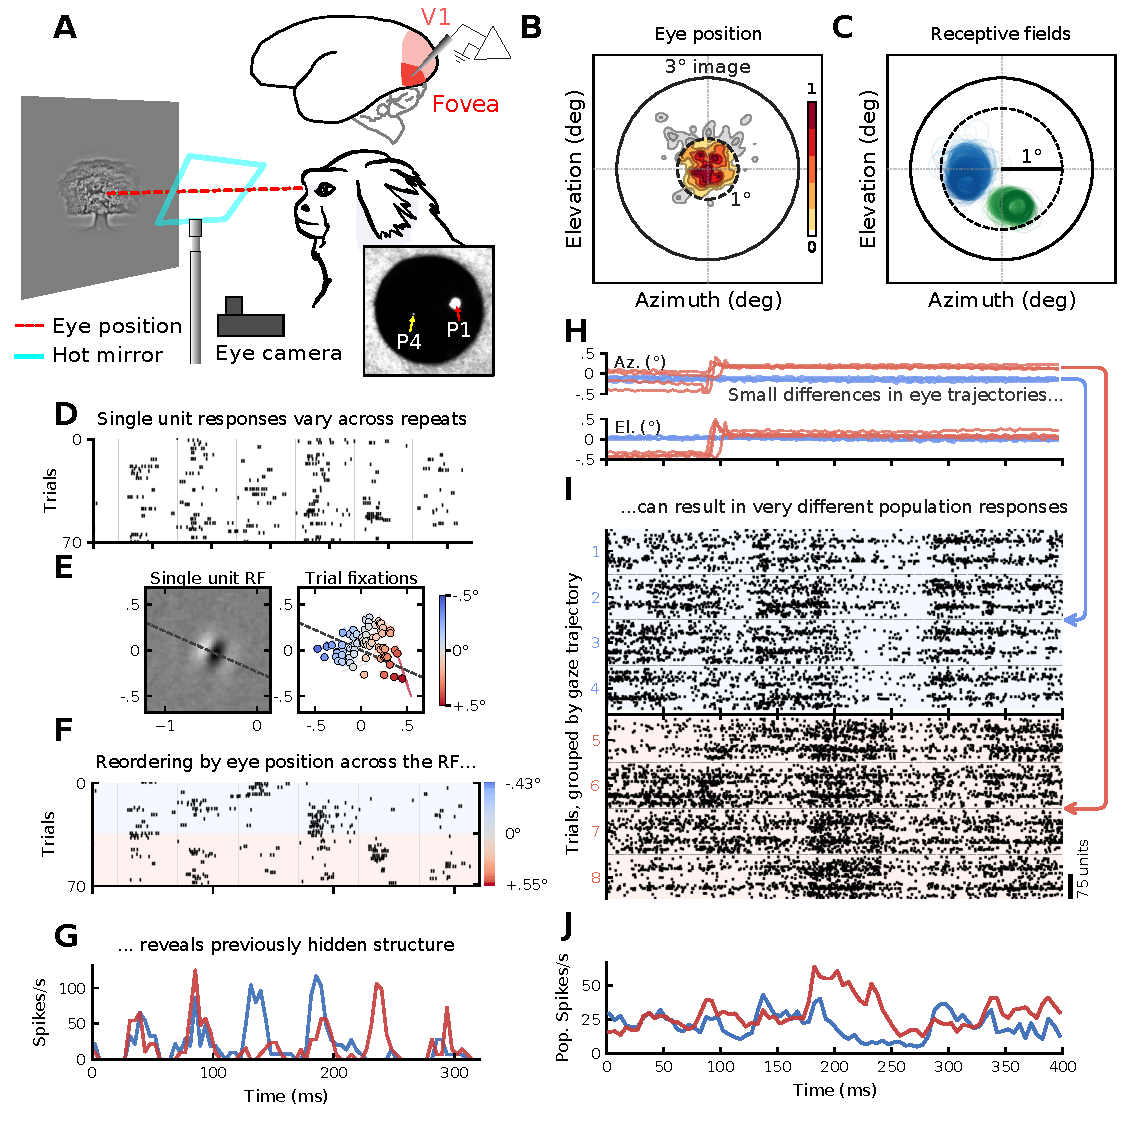
\includegraphics[width=\columnwidth]{figures/figure1.pdf} 
     \caption{
     \textbf{Small eye movements structure neural activity within the foveal representation of the primary visual cortex}
    \textbf{(A)} Schematic of the experimental paradigm. A head-fixed marmoset fixated a rapidly updating sequence of flashed images ($3^\circ$ diameter). Electrical activity was recorded using laminar probes from the lateral surface of V1. The eye's position was tracked using a high-precision digital dual Purkinje image eye tracker. The eye was imaged through a hot mirror that allowed the subject to view the stimulus. A representative image of the Purkinje images is shown in the inset.
    \textbf{(B)} Distribution of eye positions during fixation for a representative experiment. Marmosets maintained tight fixational control, which was further refined by only considering eye positions within a $1^\circ$ diameter circle for analysis.
    \textbf{(C)} Receptive field (RF) locations. The extent of each unit's RF is drawn as a contour. Blue contours represent units recorded from monkey A, and green contours from monkey L. All units had receptive fields within $1^\circ$ from the fovea.} % Optional marker
    \label{fig:fig1}
\end{figure}



%\clearpage

\begin{figure}[!t]
    \ContinuedFloat
    \caption[]{
    \textbf{(D)} Trial rasters for the example unit, ordered by trial number. The single-unit responses vary across repeated stimulus presentations. 
    \textbf{(E)} Left: The RF for the unit shown in (D), which was obtained by spike-triggered averaging. The RF displays clear, Gabor-like structure. Right: The average eye position in a 50 ms bin across trials. Points are colored according to their projection onto the line orthogonal to the subunits of the RF. 
    \textbf{(F)} Trial rasters sorted by eye position across the RF. Sorting is performed independently for each 50 ms. Smooth variation in trial-to-trial responses emerges when sorting by eye position, indicating a relation between the eye's position and the neural response. 
    \textbf{(G)} The peristimulus time histogram of responses with positive projections across the RF (blue) and negative projections (red). Average stimulus-evoked responses diverge strongly between 100 ms and 250 ms. 
    \textbf{(H)}  Eye position over time for eight representative trials colored in red and blue. The eye position traces are highly self-similar within groups, but not between groups. 
    \textbf{(I)} Population rasters for the eight representative trials from (H). There is clear similarity between population responses on trials with similar eye trajectories, and large differences between trials with dissimilar eye trajectory, despite the fact that the difference in position is just fractions of a degree. 
    \textbf{(J)} Spiking activity averaged across all recorded units for the four red trials and four blue trials over the same time course. The average population firing rate diverges strongly around 200 ms in the trial. 
    }
\end{figure}

% \clearpage

We recorded from populations of 10--118 analysis-eligible units per session (1,022 units across 19 sessions) in the foveal representation of primary visual cortex (V1) in two awake marmosets. Subjects were trained to maintain stable fixation within a 1° window while viewing a repeated sequence of rapidly flashed, whitened natural images presented at 20 Hz (Fig. 1A). Gaze position was monitored with a high-precision digital dual Purkinje image eye tracker \cite{yates2023detailed} and remained well within the fixation window across trials (Fig. 1B). These fixation distributions are similar to those observed in humans and macaques \cite{cherici2012precision, ressmeyer2025openirisdpi}. Receptive fields of recorded units were confined to eccentricities of $<$1° (Fig. 1C). As expected, activity was elicited in the recorded units by the visual stimuli presented over their receptive fields (RF), and the resulting patterns of spikes were variable from trial to trial (Fig. 1D). 

Trial-to-trial variability was strongly related to the position of the eye. For each unit we measured the displacement of the eye between trials, projected onto the axis across which the unit's receptive field is tuned (Fig. 1E, extended data figure 1). Sorting the stimulus-evoked responses by this displacement revealed clear structure in the trial-to-trial fluctuations (Fig. 1F), and splitting trials by the sign of the projection, produced markedly different response timecourses (Fig. 1G). FEMs can therefore substantially structure the activity of individual units.

Response structuring by FEMs was evident at the population level as well. We visualized population level rasters from multiple trials while conditioning on clusters of similar gaze trajectories. We identified two groups of trials with highly self-similar eye trajectories, but which differed from one other (Fig. 1H). Population responses were reproducible within each group (trials 1-4, blue), whereas trials with distinct trajectories exhibited systematically different patterns of activity (trials 5-8, red; Fig. 1I). These distinct profiles are apparent in the group-averaged population responses (Fig. 1J)-- even though the stimulus was identical across all trials. 

These visualizations make a qualitative case that FEMs structure responses at both the single-unit and population levels. A comprehensive and quantitative account requires additional statistical dissection. A simple, intuitive approach would select a subset of trials on which the eye followed nearly identical trajectories. However, such trials are rare, and collecting enough of them would exceed the duration of a typical experimental session. We therefore turned to a statistical approach that quantifies how FEMs modulate population variability without requiring exact repeats \cite{mcfarland2016variability}.



\subsection{Active sensing accounts for most residual neural variability}


\begin{figure}[p]
  \centering
  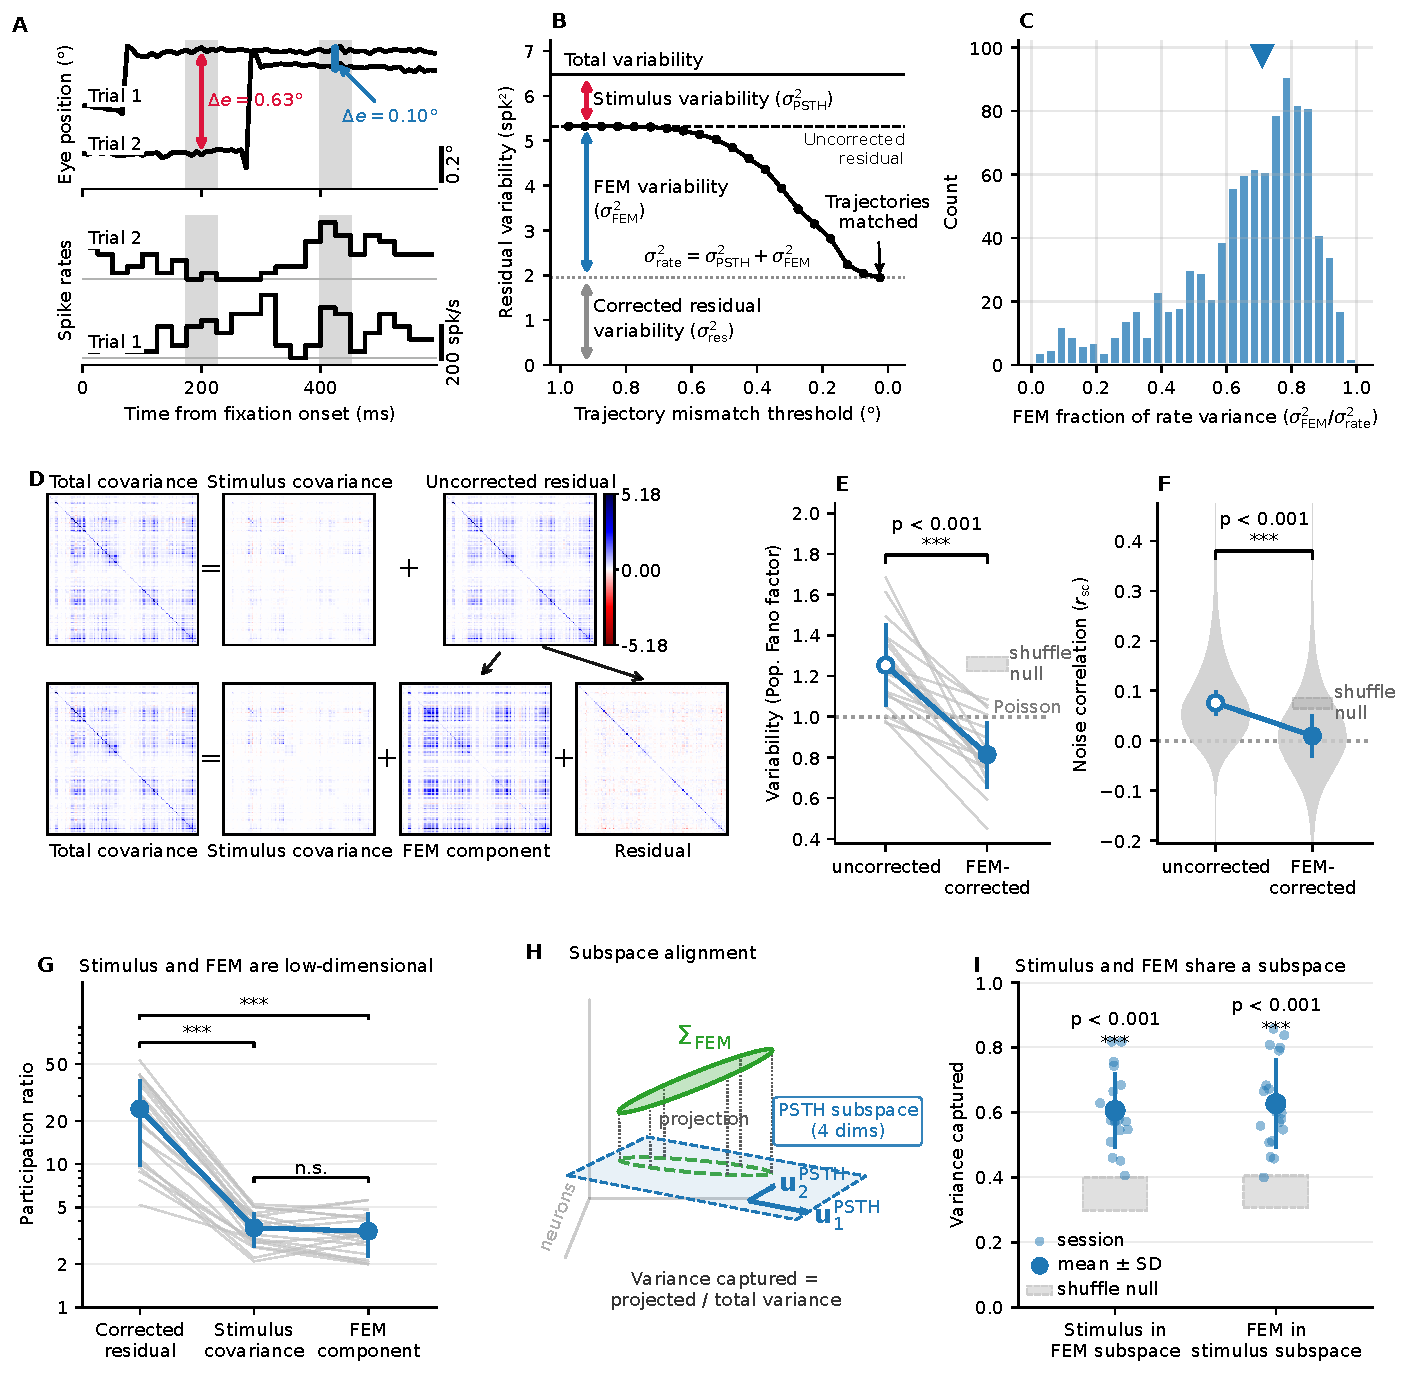
\includegraphics[width=\linewidth]{figures/figure2.pdf}
  \caption{
  \textbf{Fixational eye movements dominate single-unit and shared variability, and contribute a compact population covariance component aligned with the stimulus-driven subspace.}
  All panels use a 25\,ms counting window. Significance markers ($\ast$) denote comparison against the eye-trajectory shuffle null (E, F, I) or paired tests across components (G); numeric values are reported in the main text.
  \textbf{(A)} The comparison underlying the decomposition, for an example unit. At a fixed timepoint in the frozen stimulus sequence, eye trajectories are compared across trials. Top: eye-position traces for two trials whose eye position is closely matched at one timepoint (blue, $\Delta e = 0.10^\circ$) and divergent at another (red, $\Delta e = 0.63^\circ$). Bottom: the corresponding per-bin spike rates. Responses are similar when the eye's position is aligned across trials, while divergent eye positions yield divergent responses despite identical stimulus input.
  }
  \label{fig:covariance}
\end{figure}

% \clearpage

\begin{figure}[!t]
  \ContinuedFloat
  \captionsetup{font=footnotesize,singlelinecheck=false}
  \caption{
  \textbf{(B)} Eye-attributable variability for the same unit, recovered by tightening the matching threshold. As trial pairs are required to have increasingly similar trajectories ($\Delta e < x$), the estimate falls from the uncorrected residual toward the residual variability that survives once eye position is accounted for. The gap (blue) is the conditional rate variance attributable to fixational eye movements, and $f_{\text{FEM}}$ is the fraction of the conditional rate variance that an analysis blind to eye position would count as noise.
  \textbf{(C)} Distribution across units of the FEM fraction of single-unit conditional rate variance ($f_{\text{FEM}}$); the triangle marks the pooled median. The distribution is biased toward one (median $\FigTwoFemMedian$, 95\% CI $\FigTwoFemCI$), indicating that most trial-to-trial rate variance is attributable to fixational eye movements.
  \textbf{(D)} Covariance decomposition for an example session. Top: the conventional split, total covariance $= \Cpsth + \Sigma_{\text{res}, \text{unc}}$, assigns all covariance not captured by the PSTH to a single component. Bottom: that uncorrected residual is further partitioned into an eye-movement--dependent component $\Cfem$ and a residual $\Sigma_{\text{res}}$. Off-diagonal structure in the uncorrected residual migrates almost entirely into $\Cfem$, leaving $\Sigma_{\text{res}}$ near-diagonal.
  \textbf{(E)} Population Fano factor, uncorrected vs.\ FEM-corrected. Thin grey lines are individual sessions; the marker is the across-session mean $\pm$ SD. The Poisson reference (Fano $=1$) is dotted and the grey band is the shuffle null.
  \textbf{(F)} Per-pair noise correlation, uncorrected vs.\ FEM-corrected. Grey violins show the pooled per-pair distribution; the marker is the across-session mean $\pm$ SD and the grey band the shuffle null.
  \textbf{(G)} Participation ratio of the three covariance components --- residual ($\Sigma_{\text{res}}$), stimulus-locked ($\Cpsth$), and eye-movement--dependent ($\Cfem$). One faint line per session joins its three values; the marker is the across-session mean $\pm$ SD (log scale). The stimulus and FEM components are comparably low-dimensional and far more compact than the residual.
  \textbf{(H)} Schematic of the subspace-alignment test. The low-rank FEM covariance (green disk) is projected orthogonally onto the leading eigenvectors of $\Cpsth$ (the stimulus subspace, blue plane); the fraction of variance retained, $f_{\mathrm{FEM}\to\mathrm{PSTH}} = \mathrm{tr}(U^\top\Cfem U)/\mathrm{tr}(\Cfem)$, measures how much of one component lies within the other's subspace. This is one of the two directions shown in (I), and is distinct from $f_{\text{FEM}}$ in (B, C).
  \textbf{(I)} Variance captured in each direction --- stimulus-locked variance lying in the FEM subspace, and FEM variance lying in the stimulus subspace --- with one point per session and the across-session mean $\pm$ SD. The grey dashed band is the shuffle null of the mean (the eye-trajectory shuffle). Both directions sit well above the null, indicating that FEM-driven modulation is largely confined to the dimensions used to encode the stimulus.
  }
\end{figure}
To quantify the contribution of FEMs to neural variability, we extended a recently developed method for variability decomposition (\cite{mcfarland2016variability}; Methods). Because the same time-varying image is presented on every trial, any two trials share the same stimulus at a given timepoint and differ only in the eye's position during the preceding moments. The similarity of their recent eye trajectories therefore determines whether the two spike counts arose from the same retinal input (Fig.~2A). We therefore estimated variability from only those trial pairs whose recent trajectories fell within a given distance of one another, and varied that distance (Fig.~2B). When the distance is large enough to admit every pair, the estimate recovers the eye-position-blind residual, which is the variability that remains once the trial-averaged response is subtracted. As the distance shrinks, only pairs whose eye positions nearly coincided over the preceding moments contribute, and the estimate falls toward a floor. The gap between the uncorrected residual and that floor is the variability driven by fixational eye movements, and the floor is the residual variability that survives once eye position is accounted for.

We define the conditional rate variance ($\sigma^2_{\text{rate}}$) as the total variance accounted for by matching trials at the same timepoint on their recent eye trajectories. It combines the variance of the trial-averaged response ($\sigma^2_{\text{PSTH}}$) and the trial-to-trial variance attributable to differences in the eye's position ($\sigma^2_{\text{FEM}}$). 
From these we computed the fraction of the conditional rate variance attributable to fixational eye movements, $f_{\text{FEM}}$ (Fig.~2B), which had a median of $\FigTwoFemMedian$ across the population (IQR $\FigTwoFemIQR$; $n=\FigTwoFemUnits$ units; Fig.~2C). Foveal responses therefore varied more with trial-to-trial differences in eye position than with the stimulus itself, despite tight behavioral control. 

Conventional measures of neural variability compare each trial to the trial-averaged response, so anything the eye contributes is counted as noise ($\sigma^{2}_{\text{res},\mathrm{unc}} = \sigma^2_{\text{FEM}} + \sigma^2_{\text{res}}$). The decomposition instead yields an estimate of residual variability unbiased by differences in the eye's position between trials. This lowered estimates of the population Fano factor from $\FigTwoFanoUncorrected$ to a sub-Poisson value of $\FigTwoFanoCorrected$ (equal-session means) (a reduction absent under a trajectory-shuffle null, empirical $p \leq 0.001$; Fig.~2E). Units in foveal V1 are therefore less variable than the conventional residual implies.

The decomposition additionally yields the conditional rate covariance (``noise correlation") across simultaneously recorded units, via the law of total covariance (Methods). Doing so partitions the total covariance into a stimulus-locked component ($\Cpsth$), an eye-movement--dependent component ($\Cfem$), and a residual ($\Sigma_{\text{res}}$), where the conventional residual is the sum of the latter two ($\Sigma_{\text{res}, \text{unc}} = \Cfem + \Sigma_{\text{res}}$; Fig.~2D). Under this decomposition the off-diagonal structure present in the conventional residual migrated almost entirely into $\Cfem$, leaving $\Sigma_{\text{res}}$ near-diagonal. As a result, noise correlations fell from $\FigTwoNCUncorrected$ (95\% CI $\FigTwoNCUncorrectedCI$), comparable to previous reports \cite{smith2008spatial, mitchell2009spatial}, to $\FigTwoNCCorrected$ (95\% CI $\FigTwoNCCorrectedCI$), an interval including zero ($\Delta r = \FigTwoNCDifference$ (95\% CI $\FigTwoNCDifferenceCI$) vs.\ a shuffle null of $\FigTwoNCNullCI$, empirical $p \leq 0.001$; Fig.~2F). Differences in eye position across trials thus account for almost all of the shared variability left by the trial-averaged response.

The FEM-driven covariance was also low-dimensional. Its participation ratio averaged $\FigTwoPRFem$ across sessions, roughly seven-fold more compact than the residual ($\FigTwoPRResidual$) and not detectably different from the stimulus-locked covariance $\Cpsth$ ($\FigTwoPRStimulus$; sign test, 12 of 19 sessions, $p = \FigTwoPRSignP$; Fig.~2G). With both components confined to a few dimensions, $\Cfem$ could occupy the subspace that carries the stimulus response or lie orthogonal to it. Either arrangement is plausible, and each implies a different account of how V1 represents retinal displacement. A unit responds to the image falling on its receptive field, and moving the eye across a static scene changes that image much as changing the stimulus would. By that account, FEM-driven modulation would land on the dimensions the stimulus response already uses. Alternatively, the cortex could separate the content of a scene from its position on the retina, confining retinal translations to dimensions the stimulus response does not use. Models that recover fine spatial detail under fixational motion have proposed that V1 implements this separation \cite{pitkow2007neural, anderson2020high}.

These two possibilities differ in what FEM-driven variability costs the population code. Variability confined to the stimulus-encoding dimensions cannot be averaged away by pooling more units, because it grows with the population the same way the signal does, and it therefore bounds the information the population carries \cite{zohary1994correlated, moreno2014information}. Variability in orthogonal dimensions, however, would be removed by that same pooling operation. A cortex that orthogonalized retinal translation would therefore keep the stimulus code insulated from the eye's own motion.

We distinguished between these possibilities by projecting each covariance component onto the leading eigenvectors of its counterpart and computing the fraction of variance retained. The measure approaches one when the two components share a subspace and zero when they are orthogonal (Fig.~2H; Methods). It is asymmetric, so we evaluated both directions, each against a shuffle null that destroyed the trial-specific coupling between eye position and population activity. A majority of the stimulus-driven variance fell within the FEM subspace ($\FigTwoStimInFem$), and a majority of the FEM-driven variance fell within the stimulus subspace ($\FigTwoFemInStim$), each well above its shuffle null ($\approx 0.35$; $p \leq 0.001$ for both directions; Fig.~2I). FEM-driven modulation is therefore largely confined to the same low-dimensional subspace that carries the population's stimulus response.


%\clearpage

\subsection{Active visual sensing is implemented via an eye-brain-environment feedback loop}


\begin{figure}[p]
  \centering
  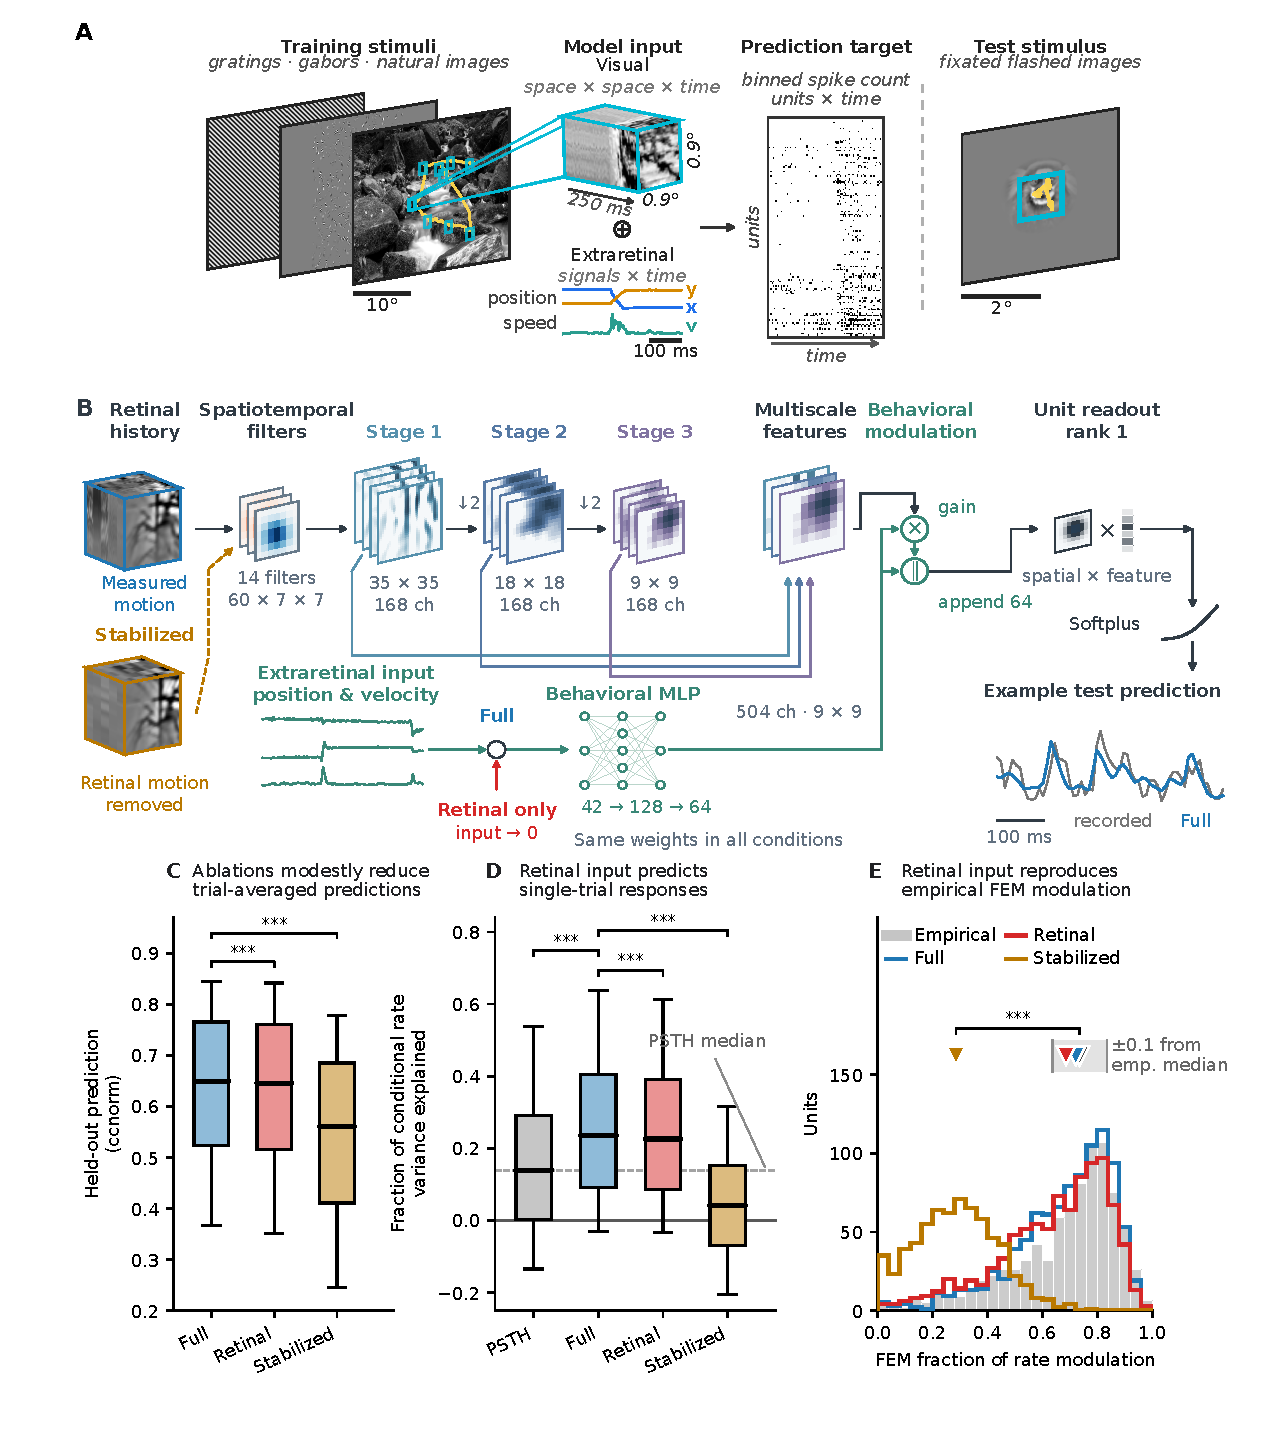
\includegraphics[width=\linewidth]{figures/figure3.pdf}
  \caption{
  \textbf{An image-computable model reproduces eye-movement driven variability through feedforward computation on retinal input}
    } % Optional marker
    
\end{figure}
\begin{figure}[t]
  \ContinuedFloat
  \captionsetup{font=footnotesize,singlelinecheck=false}
  \caption{
  \textbf{(A)} Stimuli and retinal input. The model is trained on grating, Gabor, and natural image stimuli during free viewing, and evaluated on the held-out flashed image dataset. Its inputs are the gaze-contingent retinal stimulus, a space $\times$ space $\times$ time reconstruction of the stimulus history accounting for measured eye position, and separate extraretinal eye-position and eye-velocity covariates.
  \textbf{(B)} Model architecture and input interventions. A shared feedforward core combines three spatial stages into a multiscale representation, with behavioral gain and appended additive features before factorized unit readouts and a softplus link. Colored labels identify the conditions in C--E: Full (blue) retains measured retinal motion and extraretinal input; Retinal only (red) retains retinal motion but sets the extraretinal input to zero before the behavioral MLP; Stabilized (purple) removes gaze-induced retinal motion while retaining extraretinal input. All conditions use the same fitted weights. The paired input cubes illustrate a FixRSVP history with image flashes preserved. For display, stabilization uses the example trial's medoid gaze and the cubes share the same current image; the quantified ablation fixes gaze at one session-global position. Retinal histories comprise $35\times35$ pixels and 60 frames (250~ms). Feature planes show independently contrast-normalized outputs of selected channels for the displayed FixRSVP history; their depth is schematic. Stage labels give feature-map dimensions and channel counts. Filter planes show learned filters at their peak-energy lag; readout glyphs illustrate spatial--feature factorization. Separate FixRSVP examples show the eye-position and velocity traces and a held-out PSTH with recorded (gray) and Full-model (blue) rates.
    \textbf{(C)} Held-out, trial-averaged prediction (noise-normalized correlation, $\mathrm{CC}_{\mathrm{norm}}$) for the full, retinal-only, and stabilized-retina model conditions ($n=\FigThreeCUnits$ units across \FigThreeSessions{} sessions). Relative to the full model, the median paired changes were $\Delta=\FigThreeCRetinalDelta$ for retinal-only (\FigThreeCRetinalReduction\% reduction; $p=\FigThreeCRetinalP$) and $\Delta=\FigThreeCStabilizedDelta$ for stabilized-retina (\FigThreeCStabilizedReduction\% reduction; $p=\FigThreeCStabilizedP$). Percentages are relative to the full-model median; tests are paired Wilcoxon signed-rank tests.
    \textbf{(D)} Single-trial prediction as a fraction of the conditional rate variance measured in Figure~2 ($n=\FigThreeDUnits$ units across \FigThreeSessions{} sessions). Median paired changes were $+\FigThreeDFullGain$ for full minus PSTH (95\% CI $\FigThreeDFullGainCI$; $p=\FigThreeDFullGainP$), $\FigThreeDRetinalLoss$ for retinal-only minus full (95\% CI $\FigThreeDRetinalLossCI$; $p=\FigThreeDRetinalLossP$), and $\FigThreeDStabilizedLoss$ for stabilized-retina minus full (95\% CI $\FigThreeDStabilizedLossCI$; $p=\FigThreeDStabilizedLossP$). Confidence intervals and tests use the session-cluster bootstrap. The full-model gain was \FigThreeDGainPercent\% of the PSTH median; the stabilization loss was \FigThreeDLossPercent\% of the full-model median. The dashed line marks the trial-average median and the solid line marks zero captured variance. Values above one were retained because the denominator is an estimate, not a hard upper bound. Brackets in C and D show $^*p<0.05$, $^{**}p<0.01$, and $^{***}p<0.001$.
    \textbf{(E)} Distribution of the FEM modulation fraction, $f_{\mathrm{FEM}}$, for the recorded units and each model condition. Downward triangles mark distribution medians. The empirical median was $\FigThreeEEmpirical$, compared with $\FigThreeEFull$ for the full model, $\FigThreeERetinal$ for the retinal-only model, and $\FigThreeEStabilized$ for the stabilized-retina model. The shaded band shows the empirical median $\pm0.1$. Paired two-one-sided tests with this equivalence margin supported equivalence for the full and retinal-only models ($p=\FigThreeEFullTostP$ and $p=\FigThreeERetinalTostP$, respectively), but not for the stabilized-retina model ($p=\FigThreeEStabilizedTostP$). The empirical and stabilized-retina estimates differed by a median of $\FigThreeEStabilizedDifference$ (paired Wilcoxon $p=\FigThreeEStabilizedP$). In C and D, boxes span the interquartile range, median lines mark the medians, and whiskers span the 10th--90th percentiles across units.
  }
  \label{fig:model}
\end{figure}


The prior analyses show that modulation associated with FEMs occupies the same low-dimensional subspace as the stimulus response, but they do not identify the source of that modulation. Under one account, fixational eye movements displace the image on the retina and influence activity in V1 through primarily feed-forward circuits originating in the photoreceptors (i.e., reafference). Under the other, an internal signal reporting the eye's position and motion modulates V1 independently of the image on the retina (i.e., extraretinal modulation). Both accounts are consistent with the reported population geometry, but they assign the variability to fundamentally different sources.

To distinguish between these possibilities, we fit a single image-computable feedforward neural network model to the recorded V1 population. The model was trained to predict responses to gratings, Gabors, and natural images during free viewing \cite{yates2023detailed}. The fixated flashed-image condition analyzed throughout this paper was withheld from training, so the Figure~3 predictive metrics measure generalization across both stimulus and behavioral context (Fig.~3A).

The model predicts neural responses from a 250-ms retinal history through a full-history spatiotemporal convolution followed by three spatial convolutional stages and session-specific readouts (Fig.~3B). The retinal input is gaze-contingent, so fixational eye movements move the image across the model's input window. A separate feedforward pathway converts eye position and temporally filtered eye velocity into feature gains and spatially constant additive inputs. This is the only route by which eye state can affect the model's response without changing the retinal input. (``Extraretinal'' here refers to this pathway alone; the model does not identify whether an analogous biological signal arises from efference copy, proprioception, or another source). Holding the fitted weights fixed, we compared the full model against two ablated versions. In the retinal-only condition, we set the extraretinal input to zero, testing whether that pathway improves prediction once retinal image motion has been specified. In the complementary stabilized-retina condition, we froze the retinal input for every trial at one session-global gaze centroid, removing the image motion caused by fixational eye movements while the extraretinal input remained intact. Retinal image motion and eye-state signals covary on every recorded trial, so distinguishing the two accounts requires a model in which they enter as distinct inputs and can be removed one at a time.

The full model predicted trial-averaged responses with a median noise-normalized correlation of $\mathrm{CC}_{\mathrm{norm}} = \FigThreeCFull$ across $n = \FigThreeCUnits$ units from \FigThreeSessions{} sessions (Fig.~3C). Removing the extraretinal input produced a small decrease (median $\FigThreeCRetinal$; median paired $\Delta \mathrm{CC}_{\mathrm{norm}} = \FigThreeCRetinalDelta$; paired signed-rank $p = \FigThreeCRetinalP$). Stabilizing the retinal input had a larger effect (median $\FigThreeCStabilized$; median paired $\Delta = \FigThreeCStabilizedDelta$; $p = \FigThreeCStabilizedP$). The paired losses were \FigThreeCRetinalReduction\% and \FigThreeCStabilizedReduction\% of the full-model median, respectively. Much of the trial-averaged response remained predictable, motivating an assessment at the level of single trials.
% However, the effects measured in previous sections are not changes in the mean response. FEMs organize the variability around that mean, which the trial average discards.

We therefore scored each predictor on single trials as the fraction of the conditional rate variance measured in Figure~2 that it captured (Methods). We scored the leave-one-out trial average and the three model conditions on this scale, which is zero for a constant predictor and one for an ideal predictor of the conditional rate. The trial average contains the repeatable stimulus-locked response while averaging away trial-to-trial fluctuations. It captured a median of $\FigThreeDPsth$ of the rate variance, whereas the full model captured $\FigThreeDFull$ (median paired $\Delta = +\FigThreeDFullGain$, $95\%$ CI $\FigThreeDFullGainCI$; $n = \FigThreeDUnits$ units from \FigThreeSessions{} sessions; session-clustered bootstrap, Methods; Fig.~3D). The paired gain was \FigThreeDGainPercent\% of the trial-average median. The full model therefore captured structure in individual trials that was absent from the trial average.

We then tested whether this gain was driven primarily by retinal or extraretinal input. Zeroing eye position and velocity caused a small loss of captured variance (median $\FigThreeDRetinal$; median paired $\Delta = \FigThreeDRetinalLoss$, $95\%$ CI $\FigThreeDRetinalLossCI$). By contrast, stabilizing the retinal input reduced the median fraction to $\FigThreeDStabilized$, below the trial-average median (paired $\Delta = \FigThreeDStabilizedLoss$, $95\%$ CI $\FigThreeDStabilizedLossCI$). This paired loss was \FigThreeDLossPercent\% of the full-model median. Single-trial prediction therefore depended on retinal image motion, and removing the separate extraretinal input cost substantially less than removing that motion.

We then asked whether the model reproduced the FEM modulation measured directly from the recorded units, applying the Figure~2 decomposition to each condition's predicted rates (Methods). The full and retinal-only models had medians of $\FigThreeEFull$ and $\FigThreeERetinal$, compared with an empirical median of $\FigThreeEEmpirical$. Paired equivalence tests supported agreement within a $\pm0.1$ margin (TOST $p = \FigThreeEFullTostP$ and $p = \FigThreeERetinalTostP$, respectively; Fig.~3E). Stabilizing the retinal input shifted the model median to $\FigThreeEStabilized$, outside that margin (median paired empirical-minus-model difference $\FigThreeEStabilizedDifference$; paired signed-rank $p = \FigThreeEStabilizedP$). Retinal image motion was therefore sufficient to reproduce the magnitude of FEM-driven rate modulation, and removing that motion cut it by more than half.

These results provide strong evidence that the FEM-dominated foveal code is a reafferent signature of active sensing. Fixational eye movements shape V1 activity by continuously moving the image across the retina. Within the model, retinal image motion alone was sufficient to retain the single-trial explanatory advantage when the extraretinal pathway was removed. With the retinal image stabilized and the extraretinal input intact, prediction fell below the trial-average baseline.

%\clearpage

\subsection{Fixational eye movements sharpen spatial population codes}

The preceding analyses showed that fixational eye movements (FEMs) drive large, predominantly reafferent changes in foveal V1 activity. Once gaze was accounted for, little shared variability remained. This raises a question: if shared variability is driven by FEMs, what does the retinal motion itself do to the visual representation? This cannot be measured directly in the recorded neurons for two reasons. First, the experiment provides no way to observe the same population under the counterfactual condition in which retinal motion is removed or otherwise manipulated. Second, no experimental technique can record from complete populations of cortical neurons, so any population-level account necessarily requires inference about neurons we did not record from. We therefore used the fitted encoding model both to construct complete spatial populations and to interrogate counterfactual eye movements directly. 

For each fitted unit, we replicated its spatial readout across the modeled visual field, producing a pseudo-population of identically tuned units that differed only in receptive-field position (Fig. 4A). The resulting activation map describes how selectively that feature is represented across space. We quantified this spatial selectivity using single-spike information (SSI; Methods), which measures spatial information per predicted spike, and compared activation maps generated by measured fixation trajectories with matched movies in which the retinal input was stabilized.

Measured retinal motion increased both the strength and the spatial selectivity of the model population response. In the illustrative example in Fig.~4A, the moving image produced both a higher firing rate and a more concentrated activation map than the same image held stationary on the retina. Across the population, firing rate and SSI generally increased with fixation path length, with smaller differences between the two longest-path bins (Fig.~4B). In the sixth of eight equal-count path-length bins (median \FigFourPath{} arcmin), measured motion increased firing rate by \FigFourRateEffect\% (95\% CI $\FigFourRateCI$) and SSI by \FigFourSSIEffect\% (95\% CI $\FigFourSSICI$) relative to stabilization. Thus, FEMs did not simply drive additional spikes: they increased the spatial information carried by each predicted spike.

What property of retinal motion produces this effect? Work by Rucci and colleagues has shown that fixational motion transforms spatial structure into temporal modulation \cite{rucci2015unsteady,kuang2012temporal}. When an image is stationary on the retina, its power lies at zero temporal frequency. Retinal translation redistributes that power into nonzero temporal frequencies, with the resulting temporal modulation depending on spatial frequency. Figure 4C shows normalized retinal power for drift windows with no detected saccade (left) and windows containing verified microsaccades below $1^\circ$ (right). The groups were defined from the eye-movement records independently of their spectra. For the same images, these fixation dynamics redistribute power across temporal frequencies. This suggests that the effect of a fixation should depend primarily on how the resulting spatiotemporal signal overlaps the tuning of the neurons receiving it.



\begin{figure}[p]
  \centering
  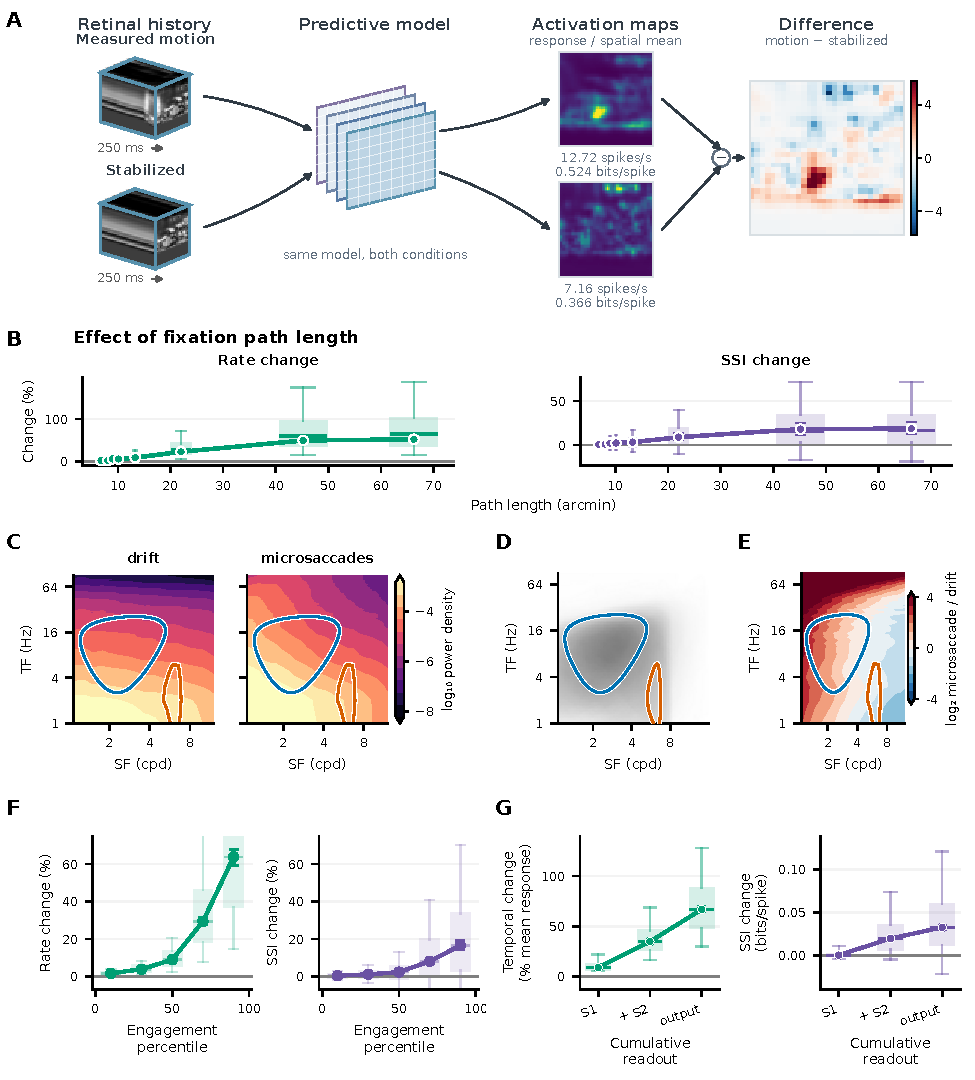
\includegraphics[width=\linewidth]{figures/figure4.pdf}
  \caption{\textbf{Fixational eye movements engage model-derived passbands and sharpen spatial coding.}}
  \label{fig:retinal_motion_passband_sharpening}
\end{figure}
\begin{figure}[!htbp]
  \ContinuedFloat
  \captionsetup{font=footnotesize,singlelinecheck=false}
  \caption{\textbf{Fixational eye movements engage model-derived spatiotemporal passbands and sharpen spatial coding in the model.}
\textbf{A}, A filtered, measured eye-movement trace and its stabilized counterpart generate 250-ms natural-image movies matched at the mean first-layer peak lag. Both movies pass through the same trained model to generate spatial activation maps for one illustrative unit. Maps show response divided by its spatial mean; the rightmost map shows motion minus stabilized. Motion increases firing rate and single-spike information (SSI) and sharpens the normalized spatial response.
\textbf{B}, Firing-rate and SSI changes versus fixation path length across \FigFourUnits{} units. Boxes show per-unit distributions; curves and error bars show population estimates and 95\% bootstrap confidence intervals.
\textbf{C}, Filled contours of equal-mass natural-image power for \FigFourDriftWindows{} drift windows and \FigFourMicrosaccadeWindows{} microsaccade-containing windows. Both conditions use one-second records filtered continuously with a positive Gaussian kernel ($\sigma=6$ ms); microsaccade amplitudes are below $1^\circ$. Each trace's nonzero-temporal-frequency power is normalized to unit mass before averaging with equal animal weights.
\textbf{D}, Model SF$\times$TF tuning for two units selected from the \FigFourValidated{} units passing strict validation. Stars mark preferred frequencies and colored contours mark fitted \FigFourPassbandPercent\%-response passbands.
\textbf{E}, Passbands for all \FigFourUnits{} model units, including \FigFourUnvalidated{} that do not pass the stricter validation criteria. Grayscale shading shows population passband occupancy; colored contours identify the validated examples in \textbf{D}.
\textbf{F}, Log$_2$ microsaccade/drift power ratio with the example passbands overlaid, illustrating how the two motion conditions engage differently tuned units.
\textbf{G}, Firing-rate and SSI modulation versus the within-unit percentile of motion-induced passband power. Greater passband engagement is associated with increases in both quantities. Boxes show unit distributions; curves show population medians with 95\% bootstrap confidence intervals.
\textbf{H}, Motion-dependent modulation across the cumulative model readout for high-passband-engagement movies. Gain-invariant temporal modulation (left) and SSI sharpening (right) increase as successive feature stages contribute to the output.
}

\end{figure}


We therefore measured the joint spatial- and temporal-frequency tuning of the matched model units using controlled drifting gratings (Fig.~4D). These units occupied a broad range of SF$\times$TF passbands (Fig.~4E). The two examples in Fig.~4D illustrate how this tuning changes the signals available to different neurons. Relative to drift windows, microsaccade-containing windows redistributed normalized natural-image power toward higher temporal frequencies, increasing the power fraction within one example passband while decreasing it within the other (Fig.~4F). Thus the same change in fixation dynamics can route retinal signals differently across V1 neurons according to their spatiotemporal tuning.

We next asked whether this tuning-specific passband engagement predicted the response to individual fixation histories. For each of the \FigFourUnits{} model units, we calculated the motion-induced power entering its joint SF$\times$TF passband across fixation trajectories. Both firing-rate and SSI modulation increased with passband engagement (Fig.~4G): the median unit effect rose from \FigFourRateEngagementLow\% in the lowest engagement quintile to \FigFourRateEngagementHigh\% in the highest for firing rate, and from \FigFourSSIEngagementLow\% to \FigFourSSIEngagementHigh\% for SSI. Within-unit Spearman correlations were larger for passband engagement than for path length (rate: median $\rho = \FigFourRatePassbandRho$ versus $\FigFourRatePathRho$, paired difference $\FigFourRateRhoDifference$, 95\% CI $\FigFourRateRhoCI$; SSI: $\FigFourSSIPassbandRho$ versus $\FigFourSSIPathRho$, paired difference $\FigFourSSIRhoDifference$, 95\% CI $\FigFourSSIRhoCI$; unit bootstrap). This is a descriptive association: the effect of a fixation depended on both its motion and how the resulting spatiotemporal signal engaged the unit's tuning.

The spectral calculation identifies which motion-generated signals enter a neuron's passband, but it does not explain how those signals become a sharper spatial representation. It describes power and discards Fourier phase, whereas the model operates on the complete spatiotemporal movie. We therefore replayed matched moving and stabilized movies through the fitted model and accumulated the trained readout contributions from successive spatial stages (Fig.~4H). Spatial sharpening was small for the first-stage contribution and larger after the second and third stages were included. These cumulative readouts reconstruct the full model output at the final stage; they describe how the trained model combines features, rather than isolating causal effects of individual stages.

\section{Discussion}

Neural activity in foveal V1 is continuously shaped by self-generated motion of the eyes, even when gaze is tightly regulated in a task that requires no sampling movement. Measuring this required tracking gaze at the scale of foveal receptive fields \cite{yates2023detailed, wu2023high} while recording dense populations of neurons. Decomposing the population covariance showed that fixational eye movements were the dominant source of rate variability in the foveal population, contributing more than the repeated sequence of natural images we presented.

Repeated presentations of stimuli are conventionally treated as repeated deliveries of the same input to the visual system. Deviations from the trial-averaged response are then thought to represent internal variability \cite{tolhurst1983statistical, shadlen1998variable}. In the fovea of alert primates, that treatment misattributes a large fraction of the residual variability, because gaze follows a different trajectory on every trial. Accounting for those trajectories lowered the population Fano factor from $\FigTwoFanoUncorrected$ to a sub-Poisson $\FigTwoFanoCorrected$ and reduced the mean pairwise correlation from $\FigTwoNCUncorrected$ to $\FigTwoNCCorrected$, consistent with the empirical summaries above. Fixational eye movements accounted for nearly all of the shared variability that the trial-averaged response did not explain.

Measured spike-count correlations span two orders of magnitude across studies, and much of that spread has been attributed to features of the preparation rather than of the circuit, including anesthetic state \cite{ecker2014state}, slow fluctuations in gain \cite{goris2014partitioning}, firing rate \cite{delarocha2007correlation}, and the counting window and spike-sorting criteria \cite{cohen2011measuring}. Recurrent excitatory--inhibitory circuits are thought to actively decorrelate neural populations \cite{renart2010asynchronous}, so remaining positive noise correlations have remained puzzling. Our results show that trial-to-trial differences in eye position can inflate estimates of noise correlation in experiments with awake animals. Fortunately, eye position differs from other factors by being readily monitored non-invasively with instrumentation that is now widely available \cite{ressmeyer2025openirisdpi}, and its influence can be accounted for with the decomposition presented here.

The eye-driven covariance was low-dimensional and lay largely within the subspace carrying the stimulus-driven response, in both directions of the alignment test. That arrangement follows from how the modulation arises. A unit responds to the image on its receptive field, and moving the eye across a static scene changes that image much as changing the display would, placing both sources of change on overlapping population dimensions. Shared variability aligned with neuronal tuning is conventionally read as a limit on the information a population carries, because a decoder cannot distinguish it from a change in the stimulus \cite{moreno2014information, kohn2016correlations}. That reading assumes the modulating variable is internal and unavailable to the readout, which fixational eye movements are not. The alignment we measured therefore specifies what a downstream stage must either know or infer to read the population correctly, rather than bounding what the population encodes.

We separated the two routes by which the eye can shape cortical activity using an image-computable model that predicted individual trials better than the cross-trial average. Removing explicit eye-position and eye-velocity signals left single-trial prediction and eye-driven modulation largely intact, whereas stabilizing the retinal input substantially reduced both. The dominant effect of FEMs in foveal V1 is therefore reafferent: the eyes change cortical activity primarily by changing the visual input itself, even though extraretinal modulation is present in some V1 neurons \cite{snodderly2001selective,kagan2008saccades}.

This reafferent origin links the apparent variability produced by FEMs to a well-established function of retinal motion. Fixational motion converts spatial structure into temporal modulation, redistributing natural-image power into the temporally band-pass regime of early visual neurons \cite{rucci2005fixational,kuang2012temporal}, and retinal stabilization impairs fine spatial vision \cite{rucci2007miniature,intoy2020finely}. Our results connect this input transformation to the cortical population code. Measured fixation trajectories produced both stronger responses and greater spatial information per predicted spike than counterfactual stabilization. Moreover, the effect depended on the interaction between the trajectory and neuronal tuning: motion-induced power entering a unit's joint spatial- and temporal-frequency passband predicted both rate and information modulation better than fixation path length alone. FEMs therefore route retinal signals through different V1 channels rather than acting as a uniform gain on the population.

The spectral redistribution describes the signal generated by FEMs, but not the full computation that produces a sharper spatial representation. The passband analysis retains power while discarding Fourier phase, whereas the fitted model operates on the complete spatiotemporal movie. Adding successive feature-stage contributions to the trained readout increased both temporal modulation and spatial information for high-engagement movies. This analysis characterizes the cumulative readout and does not isolate a causal contribution of each internal stage. Thus FEMs first make spatial structure available as a temporally modulated signal, and cortical computations further transform that signal into a more spatially informative population response. The specific spatiotemporal tuning and stagewise transformations identified here are model-derived predictions that can be tested directly with controlled dynamic stimuli.

Active vision is often considered at the scale of saccades, with each fixation treated as a static sample \cite{ballard1991animate,najemnik2005optimal,butko2010infomax,yang2016theoretical}. Our results instead show that active sensing continues throughout fixation. Movements of fractions of a degree account for much of the apparent variability in foveal V1 while simultaneously generating signals that improve spatial encoding. Foveal vision is therefore a continuous sensorimotor process in which sensor motion and neural computation operate together: the eye transforms the retinal input, cortical circuits transform the resulting spatiotemporal signal, and neural activity can in turn guide subsequent sampling \cite{vonholst1950reafferenzprinzip,gibson2014ecological,ahissar2016perception}.

\section{Methods}

\subsection{Animals and surgical preparation}

Two adult male common marmosets (\textit{Callithrix jacchus}), monkeys L and A, contributed the recordings analyzed here. The monkey L recordings were collected as part of the dataset described by Yates et al. \cite{yates2023detailed}. The monkey A recordings were collected subsequently on the same preparation and acquisition system, with the modifications noted below. The fixated flashed-image condition was not part of that report.

All surgical and experimental procedures were approved by the Institutional Animal Care and Use Committee at the University of Rochester and conformed to US National Institutes of Health guidelines. Each animal was implanted with a titanium head post and a recording chamber positioned over the foveal representation on the lateral surface of V1 \cite{yates2023detailed}.

\subsection{Eye tracking and stimulus presentation}

Animals were head-fixed during recording and viewed the display through a hot mirror. Eye position was measured with a digital dual Purkinje image eye tracker \cite{yates2023detailed, wu2023high, ressmeyer2025openirisdpi}. Visual stimuli were generated in MATLAB using Psychtoolbox \cite{kleiner2007s} and presented with a ProPixx projector (VPixx Technologies). Stimulus and electrophysiology clocks were synchronized with a Datapixx interface, which transmitted event words to the Open Ephys acquisition system. Stimulus code is available at \url{https://github.com/jcbyts/MarmoV5}.

\subsection{Fixated flashed-image condition}

Animals maintained fixation while viewing a repeated sequence of whitened natural images. Images subtended $3^\circ$ of visual angle and were presented at 20 Hz. Analyses were restricted to periods in which valid eye-position estimates remained within $0.5^\circ$ of the fixation point, a $1^\circ$-diameter fixation window. Repeated presentations of the same sequence provided matched stimulus epochs with naturally varying fixational eye trajectories.

\subsection{Free-viewing stimulus conditions}

Each session also included three free-viewing conditions taken from the foraging
paradigm described previously \cite{yates2023detailed}. No fixation was required in
these conditions. The animal viewed the display freely while stimuli were
presented continuously, and small Gabor or face targets appeared intermittently at
varying screen locations to encourage saccades. Eye position was tracked
throughout, and the stimulus falling on each receptive field was reconstructed
offline in retinal coordinates. These conditions were not used for the
variability decomposition. They provided the receptive-field estimates used to
select units for analysis, the training data for the encoding model, and the natural
free-viewing fixations analyzed in Figure~4.

\paragraph{Gabor noise.} A dense field of Gabor patches covered the display, and a
new set of patches was drawn on each noise frame, with the orientation, phase,
spatial frequency, size, and position of every patch drawn independently at random.
This condition drove units across a wide range of orientations and spatial
frequencies, and provided the data used to compute spike-triggered averages and
spike-triggered energies.

\paragraph{Gratings.} A full-field grating was presented at fixed phase and
contrast, with its orientation and spatial frequency redrawn on each noise frame.

\paragraph{Natural images.} A single natural image spanning the display was
presented on each trial and viewed freely. Fixations extracted from this condition
provided the eye-position distributions and local image measurements analyzed in
Figure~4.

\subsection{Electrophysiology and spike sorting}

Neural activity was recorded with multisite silicon electrode arrays (NeuroNexus). Each array contained two shanks separated laterally by $200~\mu\mathrm{m}$, with 32 recording sites per shank at $35~\mu\mathrm{m}$ spacing. Arrays used for monkey A were coated with poly(3,4-ethylenedioxythiophene) (PEDOT) to reduce impedance and improve signal quality \cite{cui2003electrochemical}. Wideband signals were amplified and digitized at 30 kHz with Intan headstages using Open Ephys.

Recordings from monkey L were processed and spike sorted with Kilosort 2 following Yates et al. \cite{yates2023detailed}, including manual curation in Phy. Recordings from monkey A were processed with an updated pipeline and spike sorted with Kilosort 4 \cite{roth2026flexible}. Both single-unit and multi-unit clusters were considered for analysis.

Units were included if they exhibited a visually driven receptive field, defined by more than 100 spikes during receptive-field mapping and a peak spike-triggered energy SNR greater than 5. That SNR was the maximum spatial deviation of the smoothed energy map from its median, normalized by the median deviation at the earliest lag.

\subsection{Decomposition of neural variability}

Trial-to-trial variability in neural responses reflects stimulus-locked structure, variability driven by eye movements, and residual variability that remains once both are accounted for. We separate these components by applying the law of total covariance twice to the measured spike-count covariance~\cite{mcfarland2016variability}.

\subsubsection{Setup and notation}

Let $y_{i,t} \in \mathbb{Z}_{\geq 0}^{C}$ denote the spike counts of the $C$ simultaneously recorded units on trial $i$ at stimulus time $t$, and let $e_{i,t}$ denote the eye position on the same trial at the same time. Every trial repeats the same frozen stimulus sequence, so $t$ indexes the same stimulus frame across repeats. The dimension of $e_{i,t}$ is left unspecified, as it may represent eye position alone or a short trajectory history, and could in principle contain other covariates such as a second eye variable, velocity, or other potentially relevant behavioral variables.

We write $Y$ for $y_{i,t}$ treated as a random vector over trials and times. Subscripts on $\E$ and $\C$ name the variables an operator ranges over, so $\C_{i,t}(Y)$ is taken across both trials and stimulus times, while $\C_{i}(Y \mid t,e)$ is taken across trials at a fixed stimulus time and eye state. Each covariance is a $C \times C$ matrix over units whose $(c,d)$ entry is the covariance of the spike counts of units $c$ and $d$. The total population covariance is the covariance of spike counts across trials and time,
\begin{equation}
\Sigma_{\text{total}} \equiv \C_{i,t}(Y).
\end{equation}

\subsubsection{Separating residual and rate covariance}

Applying the law of total covariance while conditioning on both stimulus time $t$ and eye state $e$ yields
\begin{equation}
\C_{i,t}(Y)
= \E_{t,e}\!\left[ \C_{i}(Y \mid t,e) \right]
+ \C_{t,e}\!\left( \E_{i}[Y \mid t,e] \right).
\end{equation}

The first term averages the trial-to-trial covariance of spike counts at fixed $t$ and $e$ over all times and eye states. It is the variability that remains after conditioning on every measured external variable, which we call the residual covariance,
\begin{equation}
\Sigma_{\text{res}} \equiv \E_{t,e}\!\left[ \C_{i}(Y \mid t,e) \right].
\end{equation}

The second term is the covariance of the conditional mean spike count, $R(t,e) \equiv \E_{i}[Y \mid t,e]$, which we call the rate covariance,
\begin{equation}
\Crate \equiv \C_{t,e}(R(t,e)).
\end{equation}

The total covariance therefore separates into a residual component and a component arising from structured changes in the underlying firing rates \cite{churchland2011variance},
\begin{equation}
\label{eq:law1}
\Sigma_{\text{total}} = \Sigma_{\text{res}} + \Sigma_{\text{rate}}.
\end{equation}

\subsubsection{Separating eye-movement and stimulus-locked rate covariance}

Applying the law of total covariance a second time, now to the rate term $R(t,e)$ and conditioning only on stimulus time $t$, yields
\begin{equation}
\C_{t,e}(R(t,e))
= \E_{t}\!\left[ \C_{e}(R(t,e) \mid t) \right]
+ \C_{t}\!\left( \E_{e}[R(t,e) \mid t] \right).
\end{equation}

The first term is the variability in firing rate at a fixed stimulus frame that arises from trial-to-trial differences in eye state, which we call the fixational eye movement (FEM) covariance,
\begin{equation}
\Sigma_{\text{FEM}} \equiv \E_{t}\!\left[ \C_{e}(R(t,e) \mid t) \right].
\end{equation}

The second term depends only on the stimulus-locked mean rate,
\begin{equation}
r(t) \equiv \E_{e}[R(t,e) \mid t] = \E_{i}[Y \mid t],
\end{equation}
and is therefore driven by the frozen stimulus sequence alone. We call it the PSTH covariance,
\begin{equation}
\Sigma_{\text{PSTH}} \equiv \C_{t}(r(t)).
\end{equation}

The rate covariance therefore separates into an eye-movement component and a stimulus-locked component,
\begin{equation}
\Sigma_{\text{rate}} = \Sigma_{\text{FEM}} + \Sigma_{\text{PSTH}}.
\end{equation}

\subsubsection{Final decomposition}

Combining the two applications of the law of total covariance yields the full factorization
\begin{equation}
\Sigma_{\text{total}} = \Sigma_{\text{PSTH}} + \Sigma_{\text{FEM}} + \Sigma_{\text{res}}.
\end{equation}
The population covariance is the sum of three components: covariance driven by the stimulus-locked response, additional rate covariance induced by fixational eye movements, and residual covariance. The identity requires only that spike counts have finite second moments, and makes no parametric assumption about how firing rate depends on eye position. The further assumptions needed to estimate the three terms are given with the estimators below.

Conventional analyses define residual covariance relative to the trial-averaged response \cite{bair2001correlated,kohn2005stimulus},
\begin{equation}
\Sigma_{\text{res}, \text{unc}} \equiv \Sigma_{\text{total}} - \Sigma_{\text{PSTH}} = \Sigma_{\text{FEM}} + \Sigma_{\text{res}}.
\end{equation}
We call this quantity the uncorrected residual and $\Sigma_{\text{res}}$ the residual.

\subsection{Estimating the covariance components}

We estimated $\Cpsth$ and $\Crate$ from a common principle. For two distinct trials $i \neq j$ at the same stimulus time $t$, the residual noise is independent, so the product of their spike counts is an unbiased estimate of the product of their underlying firing rates, with the observation noise cancelling in expectation. The two terms differ only in which pairs enter the average, all same-time pairs for the stimulus-locked term and eye-position-matched close pairs for the rate term. Estimating both from the same distinct-trial products, with a shared time-bin weighting and a shared mean, lets the four terms compose exactly and treats non-stationary drift in firing rate identically across terms.

Two features of the data can bias these estimators. The first is a correlation between image content and eye position. Because eye position is distributed around a central tendency at the middle of the fixation window, trajectories are more likely to be similar near the center of that distribution, so for a single image the trajectory distance between two trials is correlated with the image features at that position. We protect against this by presenting many images rapidly, so that no feature is consistently paired with the center of the fixation window. The second is slow drift in firing rate, which changes the sample mean across time for reasons unrelated to the stimulus or eye movements. We estimated $\Cpsth$ and $\Crate$ against a single global mean, computed under the same pair-count time-bin weighting and shared by both terms, so that drift contributes identically to both and cancels in their difference, $\hat{\Sigma}_{\mathrm{FEM}} = \hat{\Sigma}_{\mathrm{rate}} - \hat{\Sigma}_{\mathrm{PSTH}}$.

Such drift is nonetheless consequential for the correlations we report. Because close pairs are matched on eye trajectory rather than on proximity in recording time, shared slow fluctuations survive into $\hat{\Sigma}_{\mathrm{res}}$ as well as $\hat{\Sigma}_{\text{res}, \text{unc}}$, so the FEM-corrected correlations are an upper bound and the near-zero values we obtain are conservative.

\paragraph{Consistent time-bin weighting.} Fixation durations varied across trials, so after aligning to fixation onset the number of contributing trials $n_t$ decreased across stimulus time bins. The three terms have different natural weightings over these bins: the close-pair rate estimator weights each bin by its pair count ($\propto n_t(n_t-1)/2$), a per-bin-average PSTH weights each bin equally, and the pooled sample covariance weights each bin by $n_t$. When $n_t$ varies these weightings disagree, and the resulting bias falls on the off-diagonal (cross-unit) covariance, distorting the estimated noise correlations while leaving the per-unit variance almost unchanged. We therefore pinned every term, including the mean subtracted from each, to a single pair-count weighting, so that the law of total covariance holds term by term.

\paragraph{Eye-trajectory shuffle.} We evaluated all analyses against surrogate data in which the link between eye movements and spikes was broken by permuting eye trajectories across samples, where a sample is one spike-count window from one trial at one stimulus time. The permutation breaks the pairing across both trial and time, while spike counts, $\hat{\Sigma}_{\mathrm{PSTH}}$, and the per-unit mean rates are held at their observed values. We drew 1,000 surrogates per session and recomputed $\hat{\Sigma}_{\mathrm{rate}}$, and every quantity derived from it, on each. For Fano factor, noise correlation, and subspace alignment (Fig.~2E,F,I), empirical $p$-values compare the observed across-session statistic with the corresponding surrogate distribution, using a plus-one finite-sample correction. The FEM-fraction distribution (Fig.~2C) is summarized by its pooled unit median and a 5,000-resample unit-bootstrap confidence interval; no pooled-population shuffle significance test is reported for that panel.

\subsubsection{Total covariance}
We estimated $\Ctotal$ as the sample covariance of the raw spike counts across all trials $i$ and stimulus time bins $t$, under the common time-bin weighting above,
\begin{equation}
    \hat{\Sigma}_{\text{total}} = \C_{i,t}(y).
\end{equation}
This term captures all sources of variance, including time-varying mean rates, eye-movement modulations, and Poisson-like noise. Because it pools across time and trials, it is well estimated even for units with low firing rates.

\subsubsection{Stimulus-locked covariance}
The sample covariance of the peri-stimulus time histogram (PSTH) is a biased estimate of the stimulus-locked covariance, because each trial-averaged mean still carries the sampling noise of a finite trial count. We removed this bias with the distinct-trial product introduced above \cite{sahani2003linear}. At each stimulus time bin $t$ we averaged the outer product of spike counts over all pairs of distinct trials $i \neq j$, averaged the result across time bins, and subtracted the outer product of the global mean rate $\bar{\mu}$, computed across all trials and time bins under the common weighting rather than per bin,
\begin{equation}
    \hat{\Sigma}_{\text{PSTH}} = \big\langle\, \langle y_{i}(t)\, y_{j}(t)^\top \rangle_{i \neq j} \,\big\rangle_{t} - \bar{\mu}\,\bar{\mu}^\top.
\end{equation}
Because $i$ and $j$ are different trials, their residual noise is independent and averages away, leaving an unbiased estimate of the covariance of the trial-mean rate across stimulus time.

\subsubsection{Eye-movement-dependent covariance}
We estimated $\Cfem$ indirectly, by first estimating the total rate covariance $\Crate$, which captures all variance due to time-varying firing rates, both stimulus-driven and eye-movement-driven, and then isolating the eye-movement component by subtraction,
\begin{equation}
    \hat{\Sigma}_{\text{FEM}} = \hat{\Sigma}_{\text{rate}} - \hat{\Sigma}_{\text{PSTH}}.
\end{equation}
To estimate $\Crate$ we again averaged distinct-trial products, but restricted the average to pairs whose eye trajectories nearly coincided. If two trials $i$ and $j$ follow the same eye trajectory up to stimulus time $t$, their rates conditioned on stimulus, time, and eye position are equal, so the product of their spike counts estimates the squared rate with the residual noise removed. For each time bin across pairs of distinct trials we computed the root-mean-square (RMS) distance between eye trajectories over the history window of duration $H$,
\begin{equation}
    d_{ij} = \sqrt{\frac{1}{H} \sum_{\tau=0}^{H-1} \|e_{i,t-\tau} - e_{j,t-\tau}\|^2},
\end{equation}
pooled all pairs closer than a threshold $d_{ij} < \varepsilon$ ($\varepsilon = 0.05^\circ$), and used this pool to compute an estimate of the variance conditioned on there being little difference in the eye's recent trajectory between trials,
\begin{equation}
    \hat{\Sigma}_{\text{rate}} = \big\langle\, \langle y_{i}(t)\, y_{j}(t)^\top \rangle_{i \neq j, d_{i,j} < \varepsilon} \,\big\rangle_{t} - \bar{\mu}\,\bar{\mu}^\top.
\end{equation}
The $0.05^\circ$ criterion approximated conditioning on identical trajectories. Because $\varepsilon$ is small but finite, the result is a mildly conservative estimate of the rate covariance at $d_{ij} \to 0$. As formulated, this is equivalent to the analysis used by \cite{mcfarland2016variability}.

\subsubsection{Correcting the close-pair sampling bias}
Conditioning on close pairs biases $\Crate$ when the stimulus is not spatially homogeneous. The two eye positions of a close pair are each drawn from the fixational distribution $p(e)$ and must nearly coincide, so close pairs occur in proportion to $p(e)^2$, a tighter distribution concentrated toward the center of fixation, whereas $\Cpsth$ and $\Ctotal$ average over the full viewing distribution $p(e)$. If firing rate were independent of absolute eye position, as for a spatially stationary stimulus, this would not matter, and the close-pair second moment would recover the same rate variance under either distribution \cite{mcfarland2016variability}. That condition does not hold here. At each stimulus frame the image is fixed and identical across trials, so a unit's rate depends on where the eye sits within it, and the close-pair and full distributions yield different rate variances. Combining $\Crate$ estimated over one with $\Cpsth$ and $\Ctotal$ estimated over the other breaks the factorization.

We corrected this by importance-reweighting the close-pair second moment onto the true viewing distribution. We estimated the fixational density $\hat{p}(e)$ and the density of close-pair midpoints $\hat{p}_{\text{cp}}(e)$ by kernel density estimation, and weighted each close pair at midpoint $e$ by the ratio $\hat{p}(e) / \hat{p}_{\text{cp}}(e)$, normalized across pairs and clipped to bound the influence of rarely visited positions. This maps the close-pair sampling density back to $p(e)$, so that $\Crate$, $\Cpsth$, and $\Ctotal$ are all quantified over the distribution the animal actually viewed. The correction extends the cross-trial decomposition, which assumes a spatially homogeneous stimulus, to structured stimuli whose rate variance depends on where the eye lands.

\subsection{Neural variability metrics}
Metrics were computed for units with mean firing rates above 2 spikes/s and split-half PSTH reliability $R^2 > 0.10$. Sessions with fewer than 10 qualifying units were excluded. These criteria retained a mean of $79.6 \pm 26.1$ units per session for monkey A and $18.2 \pm 9.1$ for monkey L (mean $\pm$ s.d. across sessions). Primary results used a 25-ms counting window; analyses at 8.3, 16.7, and 50 ms assessed robustness to counting-window duration.

\subsubsection{Population Fano factor}
We quantified population variability from the relation between residual spike-count variance and mean spike count across units within each recording session. For unit $c$, the uncorrected and FEM-corrected residual variances were the corresponding diagonal entries of $\hat{\Sigma}_{\text{res}, \text{unc}}$ and $\hat{\Sigma}_{\mathrm{res}}$, respectively. For each condition, the population Fano factor was the slope through the origin of residual variance $v_c$ against expected spike count $\mu_c$ \cite{churchland2010stimulus},
\begin{equation}
F = \frac{\sum_c \mu_c v_c}{\sum_c \mu_c^2}.
\end{equation}
Slopes were computed separately for each session. Figure~2E reports the mean and standard deviation across sessions. Statistical significance was evaluated against the eye-trajectory shuffle, recomputing the FEM-corrected slope within each session and comparing the observed across-session mean reduction with the surrogate distribution.

\subsubsection{Noise correlations}
Pairwise noise correlations were computed separately from $\hat{\Sigma}_{\text{res}, \text{unc}}$ and the FEM-corrected $\hat{\Sigma}_{\mathrm{res}}$. Before conversion to correlations, each covariance matrix was projected onto the positive-semidefinite cone by setting negative eigenvalues to zero. For units $c$ and $d$, noise correlation was defined as
\begin{equation}
r_{cd} = \frac{\Sigma_{cd}}{\sqrt{\Sigma_{cc}\Sigma_{dd}}}.
\end{equation}
We retained the upper-triangular entries corresponding to unique unit pairs. Correlations were averaged across pairs within each session, and session means were then averaged with equal weight across sessions. Confidence intervals were estimated with 5,000 bootstrap resamples across sessions, and the FEM-corrected minus uncorrected contrast was calculated within each session. Under the eye-trajectory shuffle, corrected noise correlations and their within-session means were recomputed and averaged across sessions, and the empirical test compared the observed across-session mean change with that surrogate distribution.

\subsection{Alignment between stimulus-locked and eye-movement covariance}
We measured whether $\Cfem$ occupied the same population dimensions as $\Cpsth$, using the 25~ms counting window of the variability metrics above. Both matrices were projected onto the positive semi-definite cone as described above and eigendecomposed, $\Cpsth = U_P \Lambda_P U_P^\top$ and $\Cfem = U_F \Lambda_F U_F^\top$, with eigenvalues in descending order. We retained the leading $k$ eigenvectors of each, $U_{P,k}$ and $U_{F,k} \in \mathbb{R}^{C \times k}$, for a population of $C$ units.

Alignment was quantified as the fraction of one component's variance lying in the other's leading subspace,
\begin{equation}
f_{\mathrm{PSTH}\to\mathrm{FEM}}(k)=\frac{\mathrm{tr}\!\left(U_{F,k}^\top \Cpsth\, U_{F,k}\right)}{\mathrm{tr}(\Cpsth)},\qquad
f_{\mathrm{FEM}\to\mathrm{PSTH}}(k)=\frac{\mathrm{tr}\!\left(U_{P,k}^\top \Cfem\, U_{P,k}\right)}{\mathrm{tr}(\Cfem)},
\end{equation}
the fraction of stimulus-locked variance captured by the FEM subspace and the fraction of FEM variance captured by the stimulus subspace. The measure is asymmetric, so we report both directions.

We set $k = 4$, matching the effective dimensionality of the two components. That dimensionality was measured by the participation ratio, $(\mathrm{tr}\,\Sigma)^2/\mathrm{tr}(\Sigma^2)$ \cite{pospisil2025revisiting}, which averaged $3.6$ for $\Cpsth$ and $3.4$ for $\Cfem$ across sessions (Figure~2G).

Significance was assessed against the eye-trajectory shuffle. Each surrogate recomputed $\hat{\Sigma}_{\mathrm{rate}}$, and with it $\Cfem$ and its eigenvectors, while $\Cpsth$ and its subspace were held at their observed values. Figure~2I reports the across-session mean $\pm$ SD against that surrogate distribution. A null built on random orientation would set a much lower bar. A random $k$-dimensional subspace captures $k/C$ of a component's variance, which averaged $0.14$ across sessions, whereas under the eye-trajectory shuffle the same measures averaged $0.35$. Testing against random orientation would therefore overstate the significance of the observed alignment.


\subsection{Encoding model}

\subsubsection{Model architecture}
The model follows a ``core-readout'' architecture \cite{wang2025foundation} with a shared feedforward visual core, a separate behavioral pathway, and session-specific readouts. The fitted rank-one model contains \ModelParameters{} parameters: \ModelVisualParameters{} in the visual core, \ModelBehaviorParameters{} in the behavioral pathway, and \ModelReadoutParameters{} in the readouts. It predicts \ModelOutputChannels{} recorded output channels across \ModelSessions{} sessions; the unit subsets entering each figure are specified separately.

\paragraph{Retinal pathway.} Gaze-corrected grayscale stimuli \cite{yates2023detailed} were center-cropped to $35\times35$ pixels and retained at their native 240-Hz sampling rate. Each prediction receives 60 frames of causal stimulus history (250~ms). Fourteen learned $60\times7\times7$ spatiotemporal filters collapse this history into a single feature map. Three subsequent spatial convolutions use 84 signed channels each and kernels of $15\times15$, $11\times11$, and $9\times9$ pixels. Group normalization and local response normalization precede a sign split and rectification, yielding 168 nonnegative channels per spatial stage. Spatial kernels are Hamming-windowed; the first-layer filters additionally use a Hann frequency mask in time and space. Between spatial stages, padded $3\times3$ pooling with stride 2 and an $L^5$ norm reduces spatial resolution. Nearest-neighbor resizing brings the three stage outputs to a common $9\times9$ grid, and their concatenation provides a 504-channel multiscale representation.

\paragraph{Extraretinal pathway.} The behavioral input contains 42 features: horizontal and vertical eye position plus 40 sign-split velocity features. Position differences are normalized, transformed with a symmetric logarithm, and projected onto ten raised-cosine basis functions per axis, with peaks spanning $30$--$200$~ms. The bases are acausal, giving this pathway access to eye velocity preceding and following the prediction time. A multilayer perceptron with 128 hidden units and GELU nonlinearities embeds the behavioral vector into 64 features. A bounded gain, $1+0.5\tanh(g)$, modulates each multiscale visual channel; the 64 behavioral features are also broadcast across space and appended as additive readout channels. The model ablations manipulate this pathway and the gaze-contingent retinal input independently.

\paragraph{Sparse factorized readouts.} Each session has separate readouts for its recorded units, initialized from Gaussian spatial masks \cite{lurz2020generalization} and subsequently optimized as sparse spatial and feature factors. The readout receives all 504 multiscale visual channels and 64 appended behavioral channels on the $9\times9$ grid. The readout has rank $R=\ModelReadoutRank$. For neuron $i$, the predicted count is
\begin{equation}
\hat r_i = \operatorname{softplus}\!\left[
 b_i + \sum_{r=1}^{R}\sum_{x,y,c}
 F_{irc}\,S_{ir}(x,y)\,G_i(x,y)\,z_c(x,y)
\right],
\end{equation}
where $z_c$ is a modulated visual or appended behavioral feature, $F_{irc}$ is a feature weight, $S_{ir}$ is a learned spatial factor, and $G_i$ is a learned Gaussian envelope shared across the neuron's factors. Each neuron therefore uses one spatial--feature product. The Gaussian center, widths, and orientation are learned. A single per-neuron bias and the softplus link produce the expected spike count in each $1/240$-s bin.

\subsubsection{Training data and evaluation protocol}
The model was fit to Gabor noise, gratings, and free-viewing natural images pooled across 30 recording sessions from the two animals. The initial trial split allocated 70\% to training, 15\% to validation, and 15\% to testing. Natural-stimulus splits remained fixed throughout fitting. During the second and third training stages, all genuine grating repeats were exposed to training and gratings were sampled with weight 16 relative to the other stimulus types. Recorded-grating capture by the final model is therefore descriptive and is not a held-out generalization result.

The fixated flashed-image condition was withheld entirely from model fitting. Figure~3 evaluates predictive accuracy on repeated natural images flashed at 20~Hz under enforced fixation, a stimulus and behavioral context absent from training. All trials passing the evaluation filters are eligible because this condition contributed no training data. Figure~4 instead uses controlled drifting-grating assays and natural-image replays through the fitted model; these counterfactual analyses characterize the model and are not additional held-out neuronal prediction tests.

\subsubsection{Training procedure}
We minimized the Poisson negative log-likelihood, evaluated only at time points passing the data filters,
\begin{equation}
    \mathcal{L} = \sum_{t} \left( \hat{r}_t - n_t \log \hat{r}_t \right)
\end{equation}
where $\hat{r}_t$ is the expected count per native time bin and $n_t$ is the observed spike count. Optimization used AdamW, a two-epoch linear warmup followed by cosine annealing, bfloat16 mixed precision, and gradient-norm clipping at 10. Batches contained 128 samples from a single session, with sessions sampled uniformly, and an epoch comprised 512 batches. Weight decay was $10^{-5}$.

The model was fitted in three training phases using seed 201. First, the visual core, behavioral pathway, and Gaussian readouts were trained from scratch for 488 epochs at an initial learning rate of $5\times10^{-4}$; the checkpoint with the best validation bits per spike is retained. Second, the shared visual and behavioral representation is frozen, and the Gaussian heads are embedded in sparse rank-one readouts while preserving their predictions at the handoff. Only the readouts are optimized for 24 epochs at $10^{-4}$, and the final checkpoint is retained to complete the prescribed sparsity schedule. Third, all components are unfrozen for 64 epochs, with a readout learning rate of $10^{-4}$ and a core learning-rate multiplier of 0.05; the best validation checkpoint is selected. Every phase uses the same Poisson objective. A weak first-layer spatial Laplacian penalty encourages smoothness.

Proximal L1 sparsity is applied only to the readout's feature and spatial weights during the second and third training phases. The feature and spatial penalty coefficients are 0.1 and 0.02, respectively. Their strengths ramp from zero to their full values over epochs 2--12 of the second phase and remain constant in the third phase. After each optimizer update, each neuron's spatial factors are normalized jointly over rank and spatial position before scalar-learning-rate L1 soft thresholding is applied to the spatial and feature weights. The learned Gaussian envelope multiplies the spatial factors; its widths are constrained to 0.75--2.0 grid pixels during these sparse-readout phases. The first training phase does not apply proximal L1.

\subsubsection{Model ablations}
We evaluated three conditions using the same fitted model weights. The full condition retained both the gaze-contingent retinal stimulus and the extraretinal eye-position and eye-velocity inputs. The retinal-only condition set the extraretinal inputs to zero while retaining the gaze-contingent retinal sequence. The stabilized-retina condition retained the extraretinal inputs but froze the retinal crop for every trial within a session at one common eye position. We defined this position as the centroid of valid eye-position samples within $0.5^\circ$ of fixation and used the recorded eye-position bin nearest that centroid to render the fixed crop. Using one session-global location prevents trial identity from remaining in the retinal input through trial-specific stabilization points.

\subsection{Model performance metrics}
We evaluated predictive performance on the withheld fixated flashed-image condition with three metrics. Noise-normalized correlation ($\mathrm{CC}_{\mathrm{norm}}$) measures trial-averaged accuracy, the captured fraction of conditional rate variance quantifies trial-by-trial predictability, and the FEM modulation fraction tests whether the model reproduces the empirical eye-movement dependence. Metrics were computed per unit on matched valid bins and summarized across the eligible units and sessions.

\subsubsection{Noise-normalized correlation}
To benchmark stimulus-locked predictive accuracy with a standard metric, we report the noise-normalized correlation coefficient $\mathrm{CC}_{\mathrm{norm}}$, matching the definition used by \cite{wang2025foundation} to enable direct comparison. Let $r$ denote the in silico prediction and $y$ the in vivo response, and let $\langle \cdot \rangle$ denote averaging across stimulus repeats (trials). Define the Pearson correlation between mean responses
\begin{equation}
\mathrm{CC}_{\mathrm{abs}}
=
\frac{\mathrm{Cov}\!\big(\langle r \rangle,\langle y \rangle\big)}
{\sqrt{\mathrm{Var}\!\big(\langle r \rangle\big)\,\mathrm{Var}\!\big(\langle y \rangle\big)}}.
\end{equation}
Following \cite{schoppe2016measuring}, an upper bound on achievable correlation given finite trial count $N$ is
\begin{equation}
\mathrm{CC}_{\max}
=
\sqrt{
\frac{\mathrm{Var}\!\big(\langle y \rangle\big)-\frac{1}{N}\mathrm{Var}(y)}
{\left(1-\frac{1}{N}\right)\mathrm{Var}\!\big(\langle y \rangle\big)}
}.
\end{equation}
We then report
\begin{equation}
\mathrm{CC}_{\mathrm{norm}}
=
\frac{\mathrm{CC}_{\mathrm{abs}}}{\mathrm{CC}_{\max}}.
\end{equation}

\subsubsection{Conditional rate variance captured on single trials}
For each unit and predictor, we quantified captured count variance as
\begin{equation}
C_{\mathrm{captured}}
=
\operatorname{Var}(Y)-\operatorname{Var}(Y-\hat{Y}),
\end{equation}
where $Y$ is the observed spike count and $\hat{Y}$ is either a model prediction or the leave-one-out trial-average prediction. The model predicts at 240~Hz. Native observed and predicted counts were summed in endpoint-aligned pairs to match the fixed 120-Hz empirical analysis grid, preserving trial boundaries and exact unit identities. We then used one-bin ($8.33$~ms) counting windows from the Figure~2 analysis within $0.5^\circ$ of fixation, each carrying the same fixed three-bin ($25$~ms) matching history that the Figure~2 decomposition applies at every counting window. This counting window is the empirical comparison resolution, not the model's native bin width. All predictors were scored on the same bins with valid responses, data filters, and predictions, and units with fewer than 50 scored windows were excluded. Before scoring, each condition's predictions were given a per-unit affine calibration, a gain and an offset fit by Poisson likelihood on the same bins. This places the conditions on a comparable count scale at the cost of in-sample optimism, applied identically to every condition.

We normalized captured variance by the unit's conditional rate variance from the Figure~2 covariance decomposition,
\begin{equation}
Q
=
\frac{C_{\mathrm{captured}}}
{\operatorname{diag}(\Sigma_{\mathrm{rate}})}.
\end{equation}
Writing the observed count as $Y = \lambda + \varepsilon$, where $\lambda = \mathbb{E}[Y \mid \text{stimulus}, \text{eye position}]$ is the conditional rate and $\varepsilon$ is the conditional residual, the residual is uncorrelated with any function of the conditioning variables. Under matched conditioning and sampling, $Q$ therefore reduces to
\begin{equation}
Q
=
1-\frac{\operatorname{Var}(\lambda-\hat{Y})}{\operatorname{Var}(\lambda)},
\end{equation}
an ordinary variance-explained coefficient whose target is the conditional rate rather than the noisy spike count. Any constant prediction scores zero, and a prediction that matches $\lambda$ up to an additive constant scores one. Because the denominator is fixed across conditions within a unit, normalization cannot reorder the conditions; it places units with different noise levels on a common scale before pooling. The denominator is an estimate from the Figure~2 decomposition on its empirical support, whereas the numerator additionally requires valid model predictions. Consequently, finite-sample estimates can fall below zero or exceed one; these values were retained rather than clipped.

Panel-D contrasts were tested with a session-clustered bootstrap. Sessions were resampled with replacement $10{,}000$ times, the units of the resampled sessions were pooled, and the median paired difference was recomputed, giving a percentile confidence interval. Sessions rather than units were resampled because units recorded together share a stimulus sequence and an eye trace. An equal-session-weight sensitivity analysis also gave intervals excluding zero for the three reported contrasts. The full model exceeded the trial average in \FigThreeDFullPositiveSessions{} of \FigThreeSessions{} session medians, and retinal stabilization reduced performance in all \FigThreeSessions{} sessions.

\subsubsection{Model FEM modulation fraction}
We computed the FEM modulation fraction for observed and model responses using the same matched close-pair estimator and fixation frame used in Figure~2,
\begin{equation}
f_{\mathrm{FEM}}
=
1-\alpha
=
1-\frac{\sigma^2_{\mathrm{PSTH}}}{\sigma^2_{\mathrm{rate}}}.
\end{equation}
The estimator was applied separately to the full, retinal-only, and stabilized model rates after alignment to the empirical analysis grid. It was run at the $25$~ms counting window Figure~2 reports, with the same three-bin matching history and close-pair criterion on RMS trajectory distance. The empirical distribution therefore measures the same quantity as Figure~2C, restricted to the eligible Figure~3 population. Single-trial captured variance above instead uses an $8.33$-ms window; neither analysis changes the model's native 240-Hz prediction rate. Distribution summaries retained finite fractions within $[0,1]$ without clipping. Equivalence was evaluated separately for each model condition on units with both empirical and model fractions in this range, using paired two-one-sided $t$ tests on the mean empirical-minus-model difference with bounds $[-0.10,0.10]$. The reported equivalence $p$-value is the larger of the two one-sided values; $p<0.05$ establishes equivalence within this margin. The stabilized comparison additionally used a paired two-sided Wilcoxon signed-rank test. These unit-level tests do not resample recording sessions; the shaded median band in Fig.~3E is a visual reference rather than the test statistic.

\subsection{Spatial information in model-derived populations}
For each of the \FigFourUnits{} fitted unit readouts, we replicated its spatial pooling over retinal position to form a population of identically tuned model units differing only in position. Each natural image patch was viewed along a measured eye trajectory and paired with a stabilized counterfactual. Recorded-unit identities were retained throughout.

\subsection{Retinal-motion replay and spatial information analysis}

\subsubsection{Fixational eye-movement histories}

Fixational eye-movement histories were extracted from the continuous free-viewing DDPI records. Eye position was placed on a uniform raw-sampling grid and filtered continuously with a symmetric positive Gaussian kernel of standard deviation 6~ms, truncated at five standard deviations. Filtering used 0.6~s of continuous padding on each side before sampling at 240~Hz. This gentle rolloff (approximately 22~Hz at $-3$~dB) was chosen near the independently measured DDPI spectral breakpoint. A positive kernel avoids introducing overshoot around monotonic rapid movements. Retinal-power spectra were also evaluated with standard deviations of 4 and 8~ms as sensitivity controls.

The candidate bank comprised 1{,}000 fixation histories sampled across all 30 recording sessions and across the observed path-length distribution. Saccade times and sample indices were aligned to the continuous DDPI records, preserving sample indices when invalid samples were excluded. Event coordinates were mapped into each session's DDPI calibration before measuring displacement. Eligible windows required valid native tracking, no unexplained rapid movement, and coverage inside the interval spanned by verified saved events. Native invalid samples and gaps were guarded by 100~ms; event boundaries were guarded by 50~ms. Histories with events of amplitude at least $1^\circ$, or with net displacement at least $1^\circ$ within 50~ms, were excluded from the subdegree-movement analysis. Each retained analysis interval contained 60 samples ($250$~ms). Eye position was centered within the analysis interval. The filtered path length was
\begin{equation}
L = 60\sum_{t=2}^{T}\lVert e_t-e_{t-1}\rVert_2,
\end{equation}
in arcmin. An independent screen flagged unlabeled rapid motion when native eye speed after 6-ms Gaussian smoothing exceeded the larger of 5~deg/s and the session median plus 21 median absolute deviations, outside verified event intervals expanded by 50~ms. Flagged histories were excluded rather than assigned a new microsaccade label. The population response analyses pooled eligible drift and microsaccade histories; the illustrative panel-A selection favored verified microsaccade windows. Panels~4C and~4F explicitly compared the two event-defined conditions.

\subsubsection{Natural-image replay population}

The replay population comprised the 725 units with exact session and cluster matches between the analysis population and the fitted checkpoint. Units were retained one-to-one using their exact session and cluster identities.

For the population response matrix, 40 natural-image patches were selected at evenly spaced positions from an independently ordered bank of 100 patches. Two hundred eligible fixation histories were selected after imposing a 350-arcmin maximum path length, with 100 histories from each animal and evenly spaced source rows within animal. Crossing images and trajectories produced 8{,}000 measured-motion movies. For each natural image, a matched stabilized movie held retinal displacement at zero. The complete behavioral input was fixed to zero in both conditions.

Each movie contained 60 scored samples at 240~Hz. The unavailable causal history preceding the first sample was filled by holding the initial gaze position fixed. The model was evaluated convolutionally over a larger retinal field, allowing each fitted neural readout to be translated over all admissible spatial positions and thereby producing a two-dimensional activation map at every time point. Model outputs are expected spike counts per 1/240-s bin. We multiplied them by 240 to express firing rates in spikes/s and summed the bin counts to obtain the expected count over each 250-ms movie.

The illustrative example in Figure~4A was selected from 12 images with the largest central image-gradient RMS, measured in the central half of the rendered field before model evaluation, using the rate, SSI, and response-map criteria specified below and was not used for population inference. Candidate 250-ms trace windows came from eligible records in the separately filtered one-second fixation bank. Up to six bounded windows per animal were crossed with the 12 candidate images and scored for all 725 units; the final example was restricted to the eight units with the strongest joint ranks of rate and SSI effects in the full population replay. Baseline rate and SSI had to be at least 0.5 spikes/s and 0.05 bits/spike. The strict display gates required rate increases of 25--200\%, SSI increases of 10--200\% and 0.02--0.25 bits/spike, a moving rate no greater than 50 spikes/s, and normalized map-RMS change of at least 0.12. The final choice maximized map-RMS change within those bounds. For this visualization, the measured and stabilized histories were aligned at the frame associated with the model's mean first-layer peak-energy lag: \FigFourExampleLagFrames{} frames, or \FigFourExampleLagMs{}~ms, before the prediction. The two histories therefore shared the retinal frame expected to contribute most strongly to the displayed response while differing in their preceding motion.

\subsubsection{Single-spike information}

Let $r_t(x)$ denote a unit's nonnegative predicted firing rate in spikes/s at spatial position $x$ and time $t$, and let $\bar r_t=\langle r_t(x)\rangle_x$. Spatial single-spike information was
\begin{equation}
I_t =
\left\langle
\frac{r_t(x)}{\bar r_t}
\log_2\!\left[\frac{r_t(x)}{\bar r_t}\right]
\right\rangle_x ,
\end{equation}
in bits per spike. This quantity is invariant to uniform multiplicative gain and therefore measures spatial response sharpening independently of mean firing-rate gain.

SSI was pooled across time using the expected spike count $\bar r_t/240$ as its weight. Population SSI was likewise pooled across images, trajectories, and units by expected spike count. Rate and SSI effects were reported relative to the matched stabilized condition:
\begin{equation}
\Delta Y = 100\,
\frac{Y_{\mathrm{motion}}-Y_{\mathrm{stabilized}}}
     {Y_{\mathrm{stabilized}}}.
\end{equation}

\subsubsection{Population response versus fixation path length}

For Figure~4B, the 200 fixation histories were divided into eight equal-count bins according to filtered path length. All 725 units and all 40 images contributed to every bin. Population firing rate was computed from total expected responses. Population SSI was computed from total spatial information divided by total expected spike count. Stabilized baselines were matched by image and unit.

The colored curves show the spike-weighted population estimand. Confidence intervals were obtained from 3{,}000 crossed bootstrap resamples of images, fixation histories, and units. The accompanying boxes show the distribution of independently calculated unit effects: the box spans the interquartile range, its center is the unit median, and the whiskers show the 5th and 95th percentiles. Units outside the whiskers remained in all population calculations.

\subsubsection{Model spatiotemporal tuning}

Spatiotemporal tuning was measured by replaying controlled drifting gratings through each unit's fitted readout at 240~Hz. Each stimulus contained the model's complete 60-frame history on a $35\times35$-pixel aperture sampled at 37.50 pixels/degree. The bank contained nine spatial frequencies from 1.072 to 15.940 cycles/degree; 14 nonzero temporal frequencies from 1 to 90.51~Hz plus a static condition; 18 motion directions spanning $360^\circ$; and 24 uniformly spaced endpoint phases. The primary assay used 0.25 Michelson contrast and was repeated at 0.125 contrast. Explicit gray-blank responses were measured for baseline subtraction. Behavior was held at zero.

For each condition, the primary response was the phase-averaged expected count per 1/240-s bin minus the gray-blank response. The preferred motion direction was selected from the acquired responses. At that direction, the complete dynamic SF$\times$TF response surface was fit with the separable and inseparable R0/R1 functions described by Yu et al.; the model was selected by their BIC comparison. The continuous preferred SF and TF were the maximum of the selected fitted surface. Displayed passband contours mark the boundary at 55\% of the fitted peak response within the probed frequency range.

The population plots included all 725 matched model units, irrespective of tuning-fit quality. Every unit produced finite preferred-frequency coordinates and a finite passband surface; \FigFourConvergedFits{} fits reported optimizer convergence and \FigFourNonconvergedFits{} finite nonconverged fits were included. Recorded gratings did not independently vary temporal frequency, so temporal-frequency values in Figure~4 refer to tuning inferred from the model assay, not directly measured biological TF tuning.

Figure~4E summarizes the population by evaluating every fitted surface on a shared logarithmic SF$\times$TF grid and counting, at each coordinate, the fraction of units whose normalized response exceeded the 55\% passband threshold. The displayed grayscale field represents this passband-occupancy fraction.

The two displayed tuning examples were chosen from a stricter subset of \FigFourValidated{} units. These units had complete exact-identity assays; phase-converged responses (24 versus 12 phases: surface correlation $\geq0.995$, SF/TF peak shifts $\leq0.51$ octaves, direction shift $\leq20.1^\circ$); positive blank-subtracted drive ($\geq0.002$ expected counts/bin); an interior, coherent raw tuning peak; and a successful full-grid Yu fit with $R^2\geq0.80$ and raw--fit peak discrepancies $\leq0.75$ octaves. At the second contrast, the surface correlation had to remain $\geq0.80$, peak shifts $\leq0.75$ octaves, direction shift $\leq40.1^\circ$, and drive $\geq0.001$ counts/bin. Recorded-neuron SF tuning additionally required at least 50 spikes, split-half correlation $\geq0.20$, a non-boundary peak, and matched-twin SF-curve correlation $\geq0.50$ with peak discrepancy $\leq1$ octave. These gates restrict the illustrative tuning examples, not the 725-unit population analysis.

\subsubsection{Retinal power redistributed by fixational motion}

The distribution-level power analysis used 100 natural-image patches and event-audited one-second epochs from an independently selected candidate bank of 200 fixation records. Windows without sufficient continuous filtering padding were discarded. Natural-image spatial power, $I(k)$, was estimated from Tukey-windowed Fourier transforms of the retinal image patches and averaged within animal before animals were weighted equally. For each fixation $X(t)$, retinal translation was represented by its exact unit-modulus carrier
\begin{equation}
q_k(t)=\exp[-i2\pi k\cdot X(t)] .
\end{equation}
The complete temporal spectrum $Q(k,\omega)$ of this carrier was estimated after temporal demeaning with two discrete prolate spheroidal tapers. Positive and negative temporal frequencies were folded together and motion directions were averaged. The expected translated-image spectrum was then obtained using the Kuang/Rucci factorization
\begin{equation}
S(k,\omega)=I(k)\,Q(k,\omega).
\end{equation}
This calculation retains the complete temporal order of each fixation.

For every fixation, the nonzero-TF power map was divided by its integrated dynamic power. Drift windows contained no detected event within the scored interval or 50~ms of either edge. Microsaccade windows contained at least one verified event with $0<\mathrm{amplitude}<1^\circ$, fully inside the scored interval with 50-ms margins. Both conditions passed the native-validity, event-coverage, and unmatched-motion checks described above. The comparison comprised \FigFourDriftWindows{} drift and \FigFourMicrosaccadeWindows{} microsaccade windows. Group assignment was based on eye-movement records, independently of retinal spectra and neural or model responses. Complete trajectories were retained within each window; this comparison is not an additive decomposition into drift and microsaccade motion. Traces were averaged within animal and the two animals were then weighted equally in each condition. Each displayed conditional spectrum therefore integrates to one and shows where dynamic power is distributed rather than how much total power is present.

Translation conserves image power. For each spatial Fourier mode, the TF=0 fraction was the squared magnitude of the mean translation carrier and the TF$>0$ fraction was its complement; their sum was verified numerically to equal one. Figure~4C shows the drift and microsaccade conditional distributions separately. Figure~4F shows their $\log_2$ microsaccade-to-drift ratio with the two example passbands overlaid.

\subsubsection{Direct passband engagement}

For Figure~4G, retinal power was computed directly from the 8{,}000 rendered movies used for the response matrix. Each movie underwent a spatial Fourier transform, removal of the temporal mean, and a two-taper temporal spectral estimate with DPSS parameters $NW=1.5$ and $K=2$. The resulting power was placed on the measured SF$\times$TF$\times$orientation grid.

For every unit, the movie-power tensor was projected onto that unit's nonnegative phase-RMS grating-response tensor across the complete measured SF$\times$TF$\times$orientation grid, normalized to unit mass. The engagement calculation used the acquired grating responses; the fitted Yu surfaces supplied the continuous preferred frequencies and display contours.

For each unit and fixation history, motion-induced passband power was the median measured-minus-stabilized projection across the 40 matched images. These values were converted to percentiles separately within each unit. Rate modulation was averaged over matched images, whereas SSI modulation was pooled over images by expected spike count. The fixation histories were divided into five within-unit passband-power percentile bins. Boxes show the distribution of unit-specific bin medians. The population curve is the median across units, with 95\% intervals from 5{,}000 bootstrap resamples of units and fixation histories within unit. The plotted effects express measured-minus-stabilized response modulation relative to the stabilized baseline.

\subsubsection{Cumulative network-stage analysis}

To trace the high-passband effect through the trained model, Figure~4H used fixation histories selected solely from the top 20\% of each unit's passband-power distribution. \FigFourStageTraces{} histories spanning the high-engagement range were crossed with \FigFourStageImages{} natural images, producing \FigFourStageMovies{} measured/stabilized movie pairs. Unit effects were summarized from the selected histories lying within that unit's top quintile.

The trained readout logits were partitioned according to the feature channels contributed by the first, second, and third spatial stages. The fixed zero-behavior contribution and readout bias were included once. Cumulative rate maps are formed from (1) the first spatial stage, (2) the first and second spatial stages, and (3) all three spatial stages, summing every readout factor associated with each included channel group. The model's softplus was applied to each cumulative logit. We verified numerically that the final cumulative map reproduced the full model output.

To remove trivial uniform gain, temporal response modulation was measured as
\begin{equation}
M =
\frac{
\sqrt{\left\langle
       [r_t(x)-\langle r_t(x)\rangle_t]^2
       \right\rangle_{t,x}}
}{
\left\langle r_t(x)\right\rangle_{t,x}
}.
\end{equation}
Figure~4H reports $100(M_{\mathrm{motion}}-M_{\mathrm{stabilized}})$ in percentage points. Spatial sharpening was the expected-spike-weighted absolute difference
$I_{\mathrm{motion}}-I_{\mathrm{stabilized}}$ in bits per spike. Unit effects were first summarized across the high-passband histories and then pooled by their population median; intervals were obtained from 5{,}000 bootstrap resamples of units.

% \subsubsection{Single-spike information}
% SSI analyses used a redundancy-resolved 100-channel model population derived from the canonical 756-channel spatial readout of the trained V1 digital twin. Each channel was a fitted model-output channel associated with a source-unit readout and evaluated convolutionally over spatial position. Redundant channels were identified from z-scored predicted activation movies over time and spatial readout location, after upstream exclusion of weak channels and consolidation to a vetted 265-representative population. The final compression used complete-linkage clustering with correlation distance, combining construction-case similarities by their minimum, and retained 100 actual representative channels: 58 grouped representatives and 42 singletons. For each multi-channel group, the representative was a medoid channel selected by its worst-case correlation with the group-mean activation movie; responses and readout weights were not averaged across members. We refer to these representative channels as model units below.

% For each model unit, image, trajectory, and time bin, the fitted model produced a two-dimensional activation map over spatial position, obtained by replicating the unit's Gaussian readout at every position in the modeled visual field. Single-spike information (SSI) measured the departure of that map from a spatially uniform response. Writing $r_t(x)$ for the predicted response at position $x$ in bin $t$ and $\bar r_t = \langle r_t(x)\rangle_x$,
% \begin{equation}
% \mathrm{SSI}_t = \left\langle \frac{r_t(x)}{\bar r_t} \log_2 \frac{r_t(x)}{\bar r_t} \right\rangle_x,
% \end{equation}
% in bits per spike. SSI is invariant to a multiplicative change in firing rate and measures only how selectively activity identifies position. For each movie--unit pair, SSI was first averaged over the 40 scored samples with expected-spike weights. Population SSI was then pooled over movies $m$ and units $u$ with the same weights; equivalently,
% \begin{equation}
% \mathrm{SSI}_{\mathrm{pop}} =
% \frac{\sum_{m,u,t} \hat n_{m,u,t}\,\mathrm{SSI}_{m,u,t}}
% {\sum_{m,u,t} \hat n_{m,u,t}},
% \end{equation}
% so that the population value is the spatial information carried per predicted spike. All reported effects are percent changes relative to a matched stabilized baseline, $100(\mathrm{SSI}_{\mathrm{FEM}} - \mathrm{SSI}_{\mathrm{stab}})/\mathrm{SSI}_{\mathrm{stab}}$.


% \subsubsection{Natural-image movie bank}
% We selected 100 natural-image windows from reviewed free-viewing fixations with valid local image measurements and local edge coherence $\geq 0.20$, and crossed them with 1{,}000 measured fixational eye-movement snippets drawn from the same free-viewing dataset, giving 100{,}000 image-by-trajectory movies. The trajectory bank was sampled across path lengths up to 350~arcmin; 200 snippets contained microsaccades and 800 were drift-only. Each movie contained 40 scored samples at $120$~Hz, whose centers spanned $0.325$~s, and the model's retinal input spanned the preceding 32 lags ($267$~ms). For every image we also rendered a stabilized counterfactual in which the same patch was held at zero retinal displacement for the same number of bins, scored through the identical model and SSI procedure. Stabilized baselines were matched to the image composition and unit selection of each plotted bin, so that differences in image identity or unit inclusion cannot appear as movement effects.

% \subsubsection{Local image structure and unit selection}
% Local structure was measured in gaze-centered patches of $1^\circ$ radius. Patches were discarded if less than 98\% fell inside the image or more than 5\% was background. From the Sobel gradients $g_x$ and $g_y$ we formed the structure tensor $J_{xx} = \langle g_x^2\rangle$, $J_{yy} = \langle g_y^2\rangle$, $J_{xy} = \langle g_x g_y\rangle$ within the patch, and defined edge coherence as
% \begin{equation}
% \frac{\sqrt{(J_{xx}-J_{yy})^2 + 4J_{xy}^2}}{J_{xx}+J_{yy}},
% \end{equation}
% with the local contour axis orthogonal to the dominant gradient axis. Coherence and contour orientation were treated as undefined when $J_{xx}+J_{yy}\leq 0$. Model units were split at $0.5$ cpd by the spatial frequency at which the model predicted their strongest response. This optimum was measured with a drifting-grating probe. At each spatial frequency, response amplitude was the phase-RMS of the unit's readout at non-zero temporal frequency, averaged across orientation and temporal frequency, and the optimum was the peak of a Gaussian fitted to that amplitude in $\log_2$ spatial frequency. Because the probe's grating window subtends few cycles at the lowest frequencies tested, this split orders units by predicted optimum rather than providing an absolute estimate of preferred spatial frequency. Preferred orientation and the orientation selectivity index were taken from a separate orientation probe at fixed phase, the index being the range of the response across orientations divided by its mean. Contour-aligned analyses additionally required a valid preferred orientation and an orientation selectivity index $\geq 0.05$, and classified each unit--image pair by the acute angle between the unit's preferred orientation and the local contour axis: aligned $\leq 15^\circ$, oblique $15$--$67.5^\circ$, orthogonal $\geq 67.5^\circ$. Because the contour axis varies across images, these populations are sets of unit--image pairs rather than fixed sets of units.

% \subsubsection{Dose curves and eye-movement decomposition}
% Path length was the summed Euclidean sample-to-sample displacement of the trajectory, in arcmin. Drift-only traces were divided into eight equal-count path bins and microsaccade-containing traces into five, with the stabilized condition plotted at zero path length. Microsaccades were detected as excursions of instantaneous eye speed above a robust median-absolute-deviation threshold estimated from valid sample-to-sample velocities; suprathreshold runs of at least one sample were treated as events, and traces with no suprathreshold event were treated as drift-only.

% For contour-relative analyses we projected each trajectory onto the contour-parallel axis $u$ and the contour-normal axis $v$, and summarized each component by its RMS excursion, the standard deviation of the centered projected position,
% \begin{equation}
% R_u = 60\sqrt{\left\langle ((e_t - \bar e)\cdot u)^2\right\rangle_t}, \qquad R_v = 60\sqrt{\left\langle ((e_t - \bar e)\cdot v)^2\right\rangle_t},
% \end{equation}
% in arcmin. We used RMS excursion rather than accumulated component path because the behavior--model comparison below showed that measured fixational behavior is better described by position spread than by path. Bins were constructed from pooled contour-normal and contour-parallel values so that the two components were compared over matched dose ranges, using pooled quantiles with an additional tail bin; the far tail above $3.8$ arcmin is omitted from the displayed panel.

% \subsubsection{Statistics for model SSI curves}
% Point estimates in each movement bin were expected-spike-weighted sums over all contributing unit--image--trajectory rows. Uncertainty was estimated by resampling images with replacement, recomputing the numerator and denominator of both the moving and stabilized population SSI from the resampled totals, and recomputing the percent change from those ratios. Confidence intervals used 10{,}000 image bootstrap resamples with seed 47 unless stated otherwise. Bootstrap $p$-values were two-sided sign-tail probabilities from the uncentered paired-difference distribution, with a plus-one finite-sample correction.

% \subsubsection{Contour-relative statistics of natural fixational eye movements}
% We analyzed reviewed fixation windows from the free-viewing natural-image condition across 30 recording sessions. Candidate windows were 128 samples long at $120$~Hz and advanced with a 16-sample stride through contiguous valid eye-position segments. Valid samples required finite eye-position estimates, valid tracker flags, and horizontal and vertical positions within $\pm12^\circ$; samples in detected microsaccades and the one-sample event padding were excluded from the fixation-window candidates. Windows were labeled by elapsed time from the previous event: early before $0.10$~s, mid from $0.10$ to $0.30$~s, and late thereafter. Figure~4 used reviewed mid- and late-phase windows, and after additionally requiring valid local image features and patches meeting the contamination criteria above, $11{,}749$ windows were retained.

% For each retained window, the local contour axis was measured at the mean eye position, and the centered eye-position cloud was projected onto axes spanning all angles from parallel to orthogonal to that axis. Spread along each axis was the RMS excursion in arcmin, averaged within four edge-coherence bins ($0$--$0.2$, $0.2$--$0.5$, $0.5$--$0.8$, $0.8$--$1$) with windows weighted by count. The orientation-scrambled reference replaced the measured relationship between the eye-position cloud and the local contour axis with randomized relative orientations, preserving the empirical clouds and coherence labels.

% To ask whether this arrangement was beneficial, we extracted the central 40-sample snippet of each window, projected the centered positions onto the contour-parallel and contour-normal axes, and converted the observed component RMS values into predicted SSI changes by piecewise-linear interpolation through the model dose curves; predictions outside the range of the model curves were excluded. The prediction for a window was the mean of its contour-normal and contour-parallel marginal predictions, not a direct model evaluation of a two-dimensional SSI surface.

% The random-rotation null rotated each snippet by an independent angle drawn uniformly from $[0,\pi)$, preserving its amplitude and temporal structure while breaking its specific alignment with the local contour. We used 256 rotations per window with seed 197. The reported match advantage is the observed prediction minus the mean rotated prediction, in percentage points of SSI change. Confidence intervals came from 10{,}000 bootstrap resamples of paired window predictions, treating retained windows as exchangeable observations.

% \subsubsection{Patch-radius sensitivity}
% To test whether the coupling between local image structure and eye movements depended on the scale at which structure was measured, we recomputed structure-tensor contour axes and coherence for gaze-centered patches of radius $0.25^\circ$, $0.5^\circ$, $0.75^\circ$, $1.0^\circ$, $1.25^\circ$, $1.5^\circ$, $1.75^\circ$, $2.0^\circ$, $2.25^\circ$, $2.5^\circ$, and $3.0^\circ$, using integral images over gradient products computed once per trial. The same contamination criteria were applied at every radius, so the retained window set was not identical across radii. For each window we estimated the principal axis of the eye-position covariance and compared it with the local contour axis through the alignment index $\cos(2\Delta\theta)$, where $\Delta\theta$ is the circular axis-angle difference. Values near $1$ indicate motion parallel to the contour and near $-1$ motion normal to it. For each radius we regressed this index on edge coherence across windows with coherence $>0.3$ by ordinary least squares. Figure~4H reports the fitted slope with 95\% confidence intervals from the regression standard error and corresponding Student-$t$ critical value.

\subsection{Data and code availability}
The data and associated analysis and modeling code will be made available upon publication.

\section{Acknowledgments}
This work was supported by NEI K99-EY037839-01 to D.P.R., NEI R01-EY030998 to J.F.M., NEI R01-EY018363 to M.R. We thank Yonatan Abrham (Mitchell Lab) for collecting some of the data used in this report. 

{\normalsize
\bibliography{refs}
}

\clearpage
\appendix
\setcounter{figure}{0} 
\renewcommand{\thefigure}{Extended Data Figure~\arabic{figure}}
% Tell the caption package to drop the default "Figure" name prefix
\captionsetup[figure]{name={}} 
\section*{Supplementary Information}

\subsection{Supplemental figures}

   \begin{figure}[p]
    \centering
    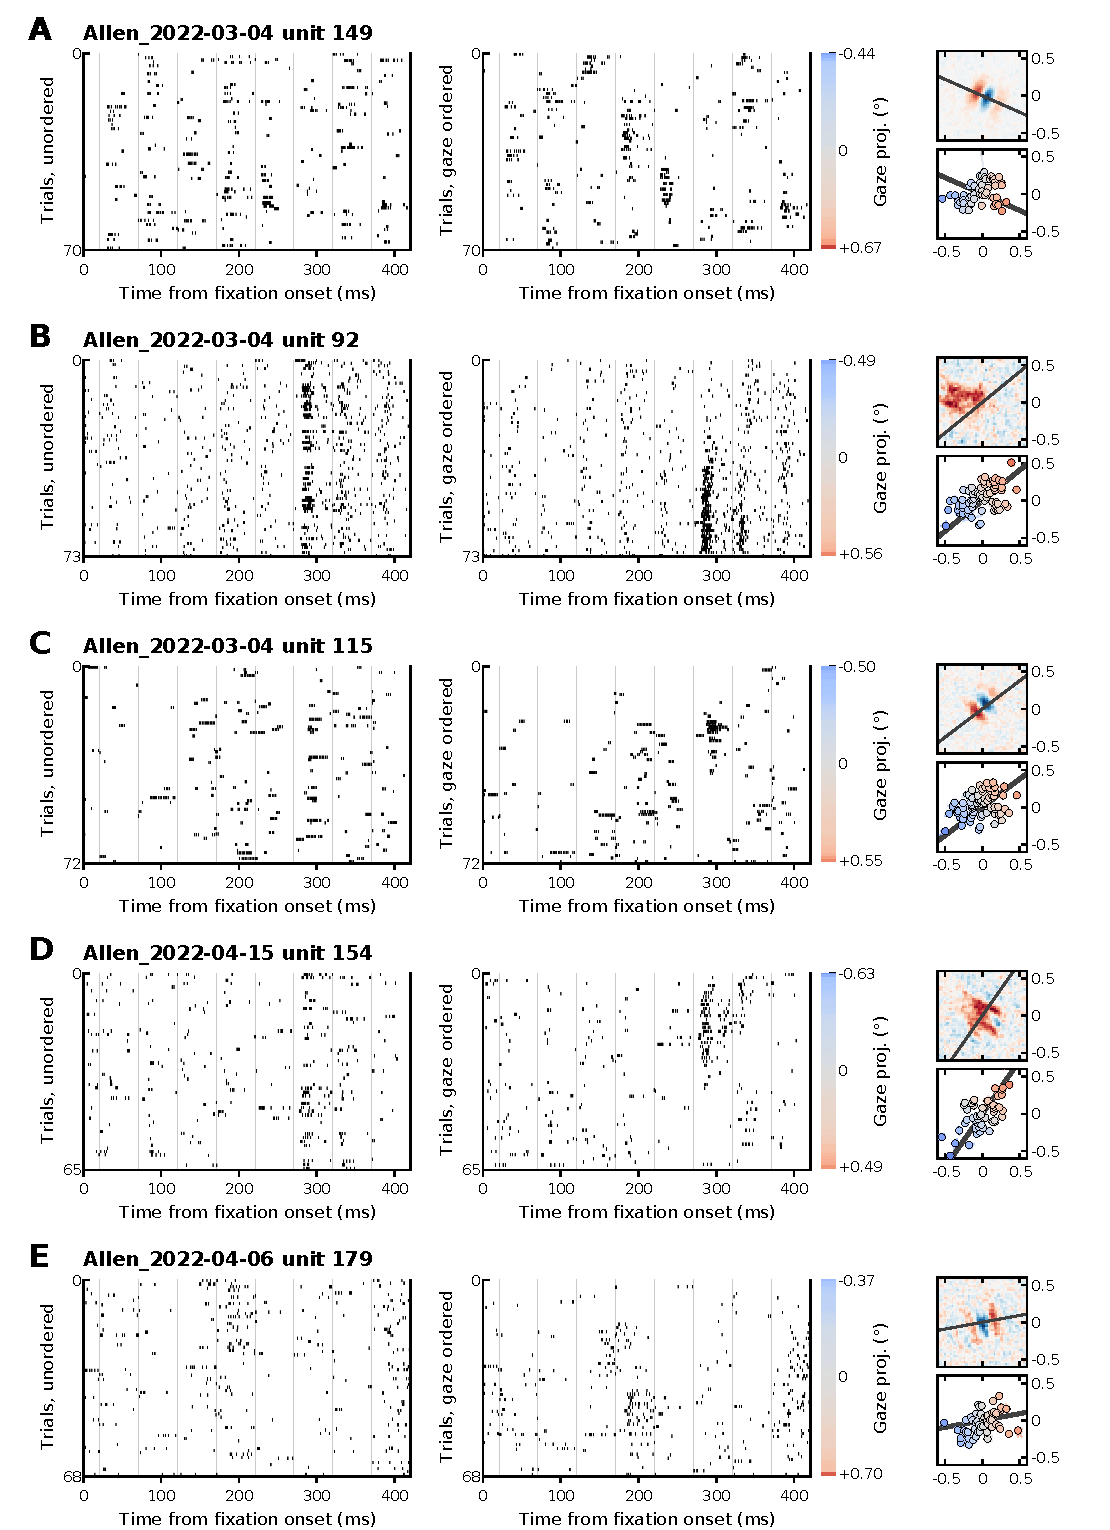
\includegraphics[width=.99\linewidth]{figures/supplement1.pdf}
    \captionsetup{font=footnotesize,skip=4pt}
    \caption{
      \textbf{Eye-position sorting reveals single-cell response structure across example V1 units.}
    }
    \label{fig:single_cell_extended}
  \end{figure}

  %\clearpage

  \begin{figure}[t]
    \ContinuedFloat
    \caption{
      Additional single-cell examples of the gaze-dependent trial structure shown in Fig.~1D--G.
      Panel \textbf{(A)} shows the same unit as Fig.~1D--G, unit 149 from Allen 2022-03-04, and includes the
      unordered trial raster for comparison.
      In each panel, left, trial rasters aligned to fixation onset with trials shown in their original unordered
      arrangement.
      Middle, the same responses reordered by gaze position projected onto the axis of maximal spatial sensitivity for that
      unit.
      Color strip, signed gaze projection for the gaze-ordered trials, with blue and red indicating opposite positions along
      the projection axis.
      Right, spike-triggered average and gaze positions for the sorting window; the black line indicates the projection axis
      used for ordering trials.
      Across units, ordering trials by eye position reveals response structure that is less apparent in the unordered
      rasters, consistent with fixational eye movements contributing to single-trial variability in foveal V1.
    }
    \label{fig:single_cell_extended_caption}
  \end{figure}
\begin{figure}[ht]
  \centering
  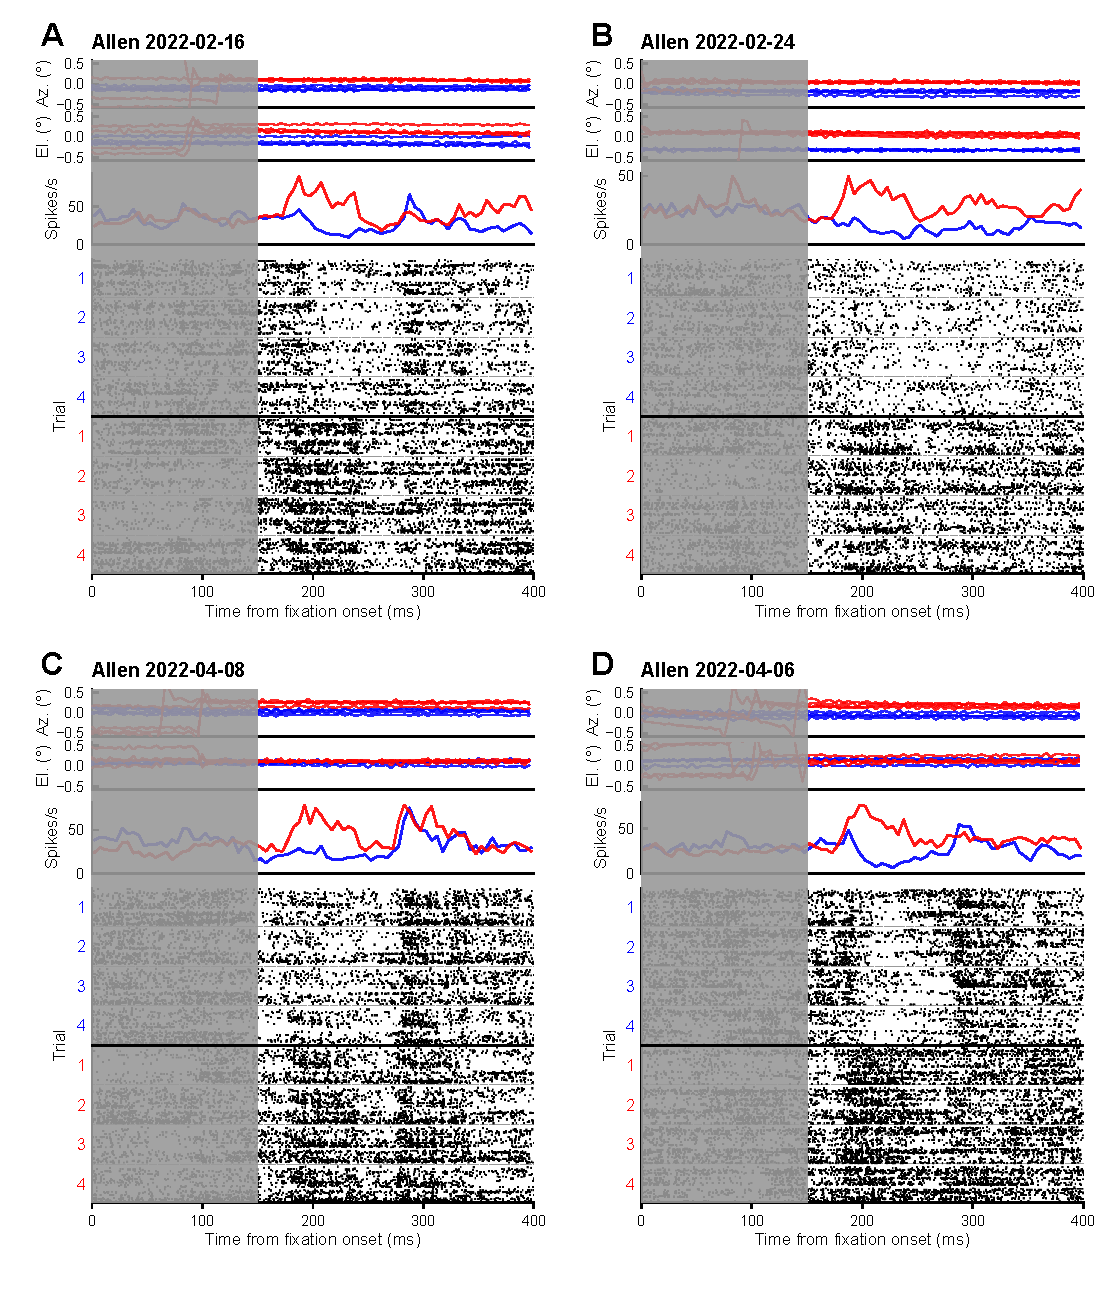
\includegraphics[width=\linewidth]{old_figures/extended_fig2.pdf}
  \caption{
    \textbf{Gaze-dependent population structure across recording sessions.}
    Additional examples of the population-level effect shown in Fig.~1H--J.
    Panels \textbf{(A)--(D)} show four sessions from monkey Allen.
    Top, horizontal and vertical gaze traces for two groups of four trials, colored blue and red; gray shading marks an initial context interval.
    Middle, population-averaged spike rate for the same trial groups.
    Bottom, population rasters for the same trials, with units stacked within trials and the black line separating blue and red groups.
    Across sessions, trials with similar gaze trajectories show similar population activity, whereas groups with distinct gaze trajectories show systematic response differences.
  }
\end{figure}
\clearpage

\end{document}
